\documentclass{beamer}
\usetheme{metropolis}           % Use metropolis theme
\usepackage{appendixnumberbeamer}
\usepackage{epigraph}
\usepackage{color}

%%% Bibliography
\usepackage[backend=bibtex, style=authoryear]{biblatex}
\bibliography{bibliography.bib}

\setbeamercolor{background canvas}{bg=white}
\setbeamercolor{title}{fg=white}
\setbeamercolor{subtitle}{fg=black}
\setbeamercolor{author}{fg=black}
\setbeamercolor{institute}{fg=white}

\newcommand{\todo}{\alert{TODO}}
\newcommand{\itemBullet}{\scriptsize$\blacksquare$}
\setbeamertemplate{itemize item}{\itemBullet}
\setbeamertemplate{itemize subitem}{\itemBullet}
\setbeamertemplate{itemize subsubitem}{\itemBullet}
\newcommand{\E}{\mathop{\mathbb{E}}}

\title{Mastering the game of Go}
\subtitle{with deep neural networks and tree search}
\date{}                         % no dates
\author{Karel Ha \\ article by Google DeepMind}
%\author{Google DeepMind \\ presented by Karel Ha}
\institute{Spring School of Combinatorics 2016}

\begin{document}
  {
    \usebackgroundtemplate{
      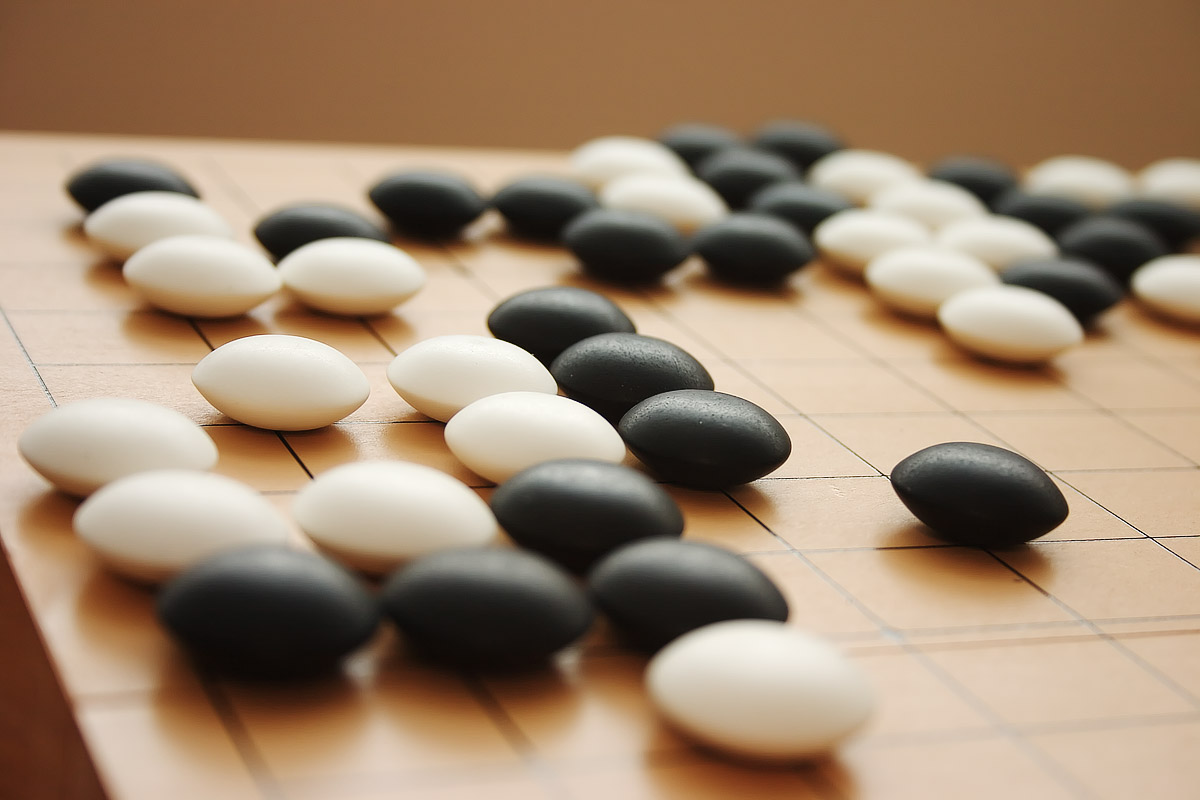
\includegraphics[height=\paperheight]{../img/Go_background.jpg}
    }
    \maketitle
  }

%%%%%%%%%%%%%%%%%%%%%%%%%%%%%%%%%%%%%%%%%%%%%%%%%%%%%%%%%%%%%%%%%%%%%%%%%%%%%%%%

  \section{Why AI?}

  \begin{frame}{Applications of AI}
    \begin{itemize}[<+- | alert@+>]
      \item spam filters
      \item recommender systems (Netflix, YouTube)
      \item predictive text (Swiftkey)
      \item audio recognition (Shazam, SoundHound)
      \item music generation (\cite{DeepHear})
      \item self-driving cars
    \end{itemize}
    \pause

    and...
  \end{frame}

  {
    \setbeamertemplate{frame footer}{\cite{Corrado15}}
    \begin{frame}{Auto Reply Feature of~Google Inbox}
      \begin{center}
        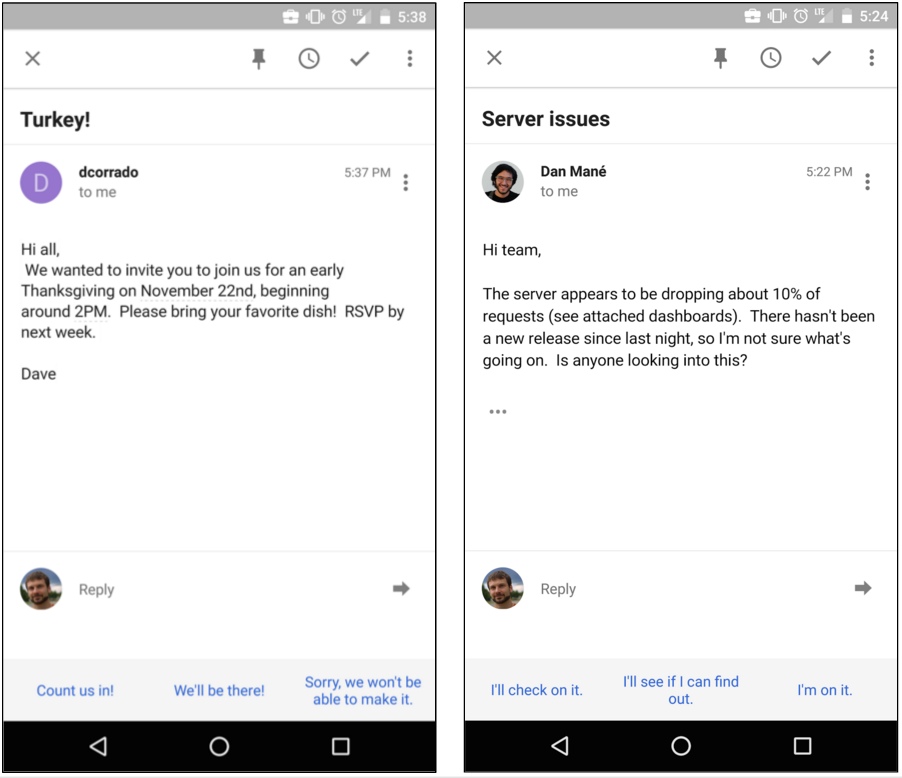
\includegraphics[height=.85\textheight]{../img/Inbox_auto_reply.png}
      \end{center}
    \end{frame}
  }

  {
    \setbeamertemplate{frame footer}{[1] \cite{GatysEB15a} [2] \cite{LiW16}}
    \begin{frame}{Artistic-style Painting}
      \begin{center}
        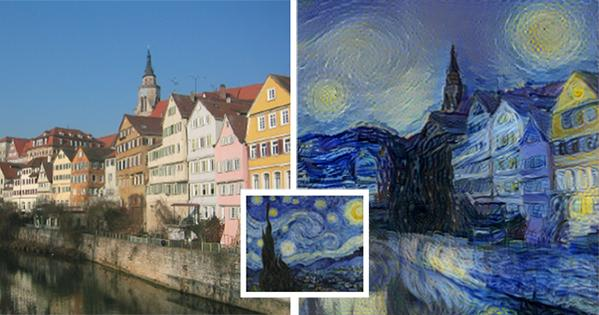
\includegraphics[height=.4\textheight]{../img/art_Van_Gogh.jpg}
        \pause

        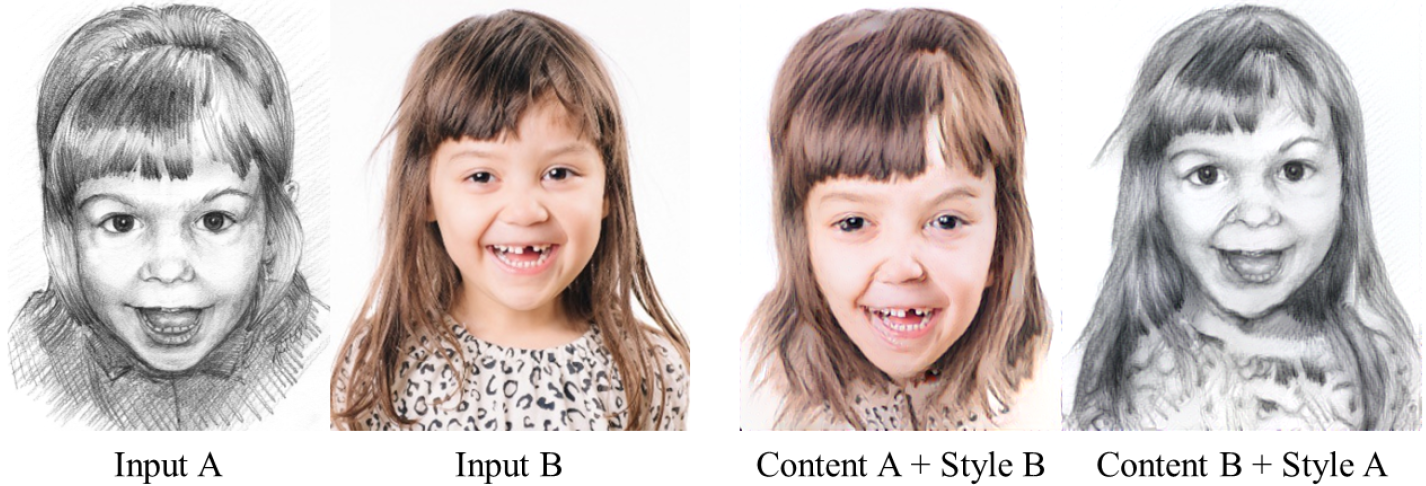
\includegraphics[height=.44\textheight]{../img/art_girl.png}
      \end{center}
    \end{frame}
  }

  {
    \setbeamertemplate{frame footer}{\cite{Karpathy15}}
    \begin{frame}{Baby Names Generated Character by Character}
      \begin{itemize}[<+- | alert@+>]
        \item Baby Killiel Saddie Char Ahbort With
        \item Rudi Levette Berice Lussa Hany Mareanne Chrestina Carissy
        \item Marylen Hammine Janye Marlise Jacacrie Hendred Romand Charienna Nenotto Ette Dorane Wallen Marly Darine Salina Elvyn Ersia Maralena Minoria Ellia Charmin Antley Nerille Chelon Walmor Evena Jeryly Stachon Charisa Allisa Anatha Cathanie Geetra Alexie Jerin Cassen Herbett Cossie Velen Daurenge Robester Shermond Terisa Licia Roselen Ferine Jayn Lusine Charyanne Sales Sanny Resa Wallon Martine Merus Jelen Candica Wallin Tel Rachene Tarine Ozila Ketia Shanne Arnande Karella Roselina Alessia Chasty Deland Berther Geamar Jackein Mellisand Sagdy Nenc Lessie Rasemy Guen
      \end{itemize}
    \end{frame}

    \begin{frame}{C code Generated Character by Character}
      \begin{center}
        \vskip -1.1ex
        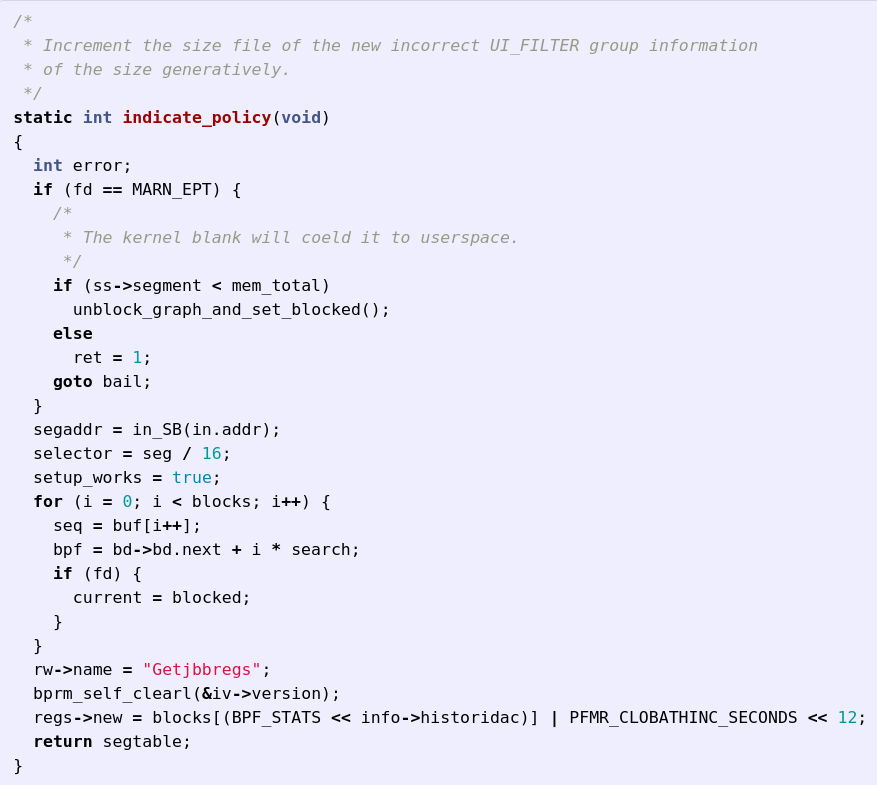
\includegraphics[height=.9\textheight, keepaspectratio]{../img/generating_c.png}
      \end{center}
    \end{frame}

    \begin{frame}{Algebraic Geometry Generated Character by Character}
      \begin{center}
        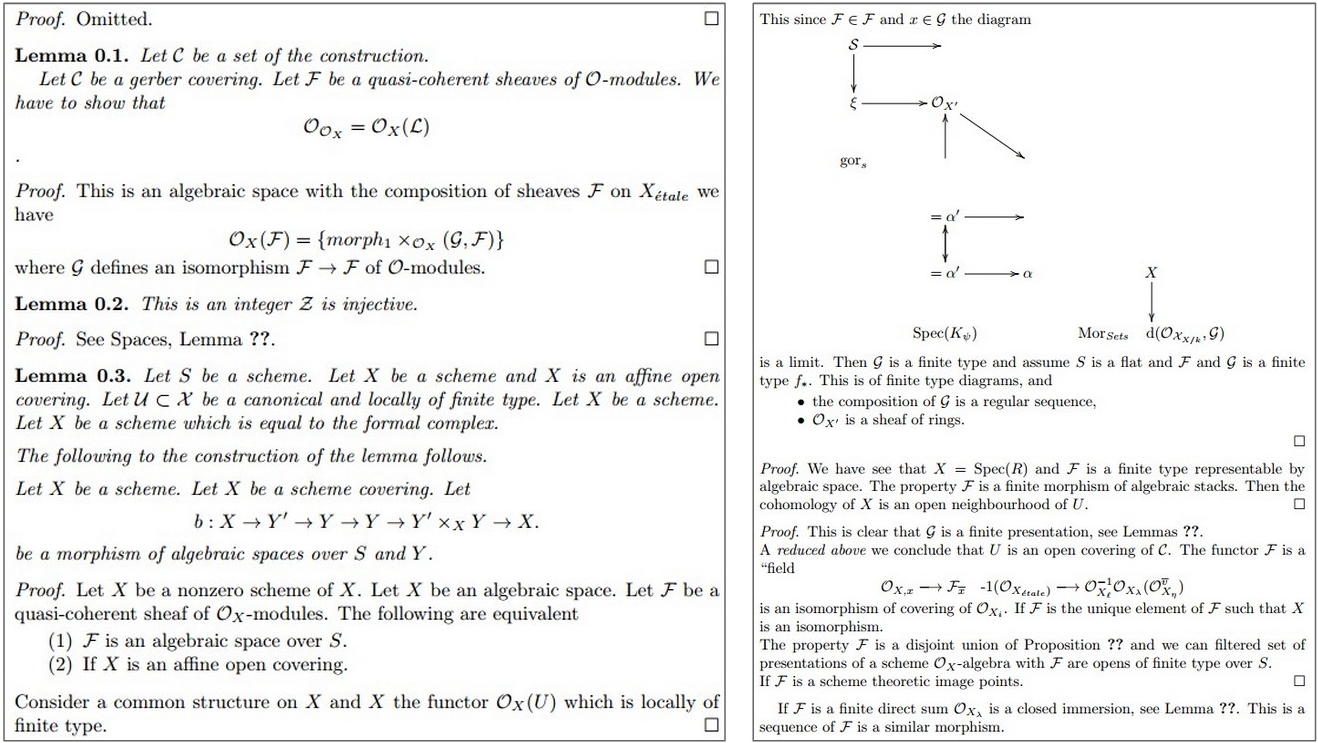
\includegraphics[width=\textwidth, height=\textheight, keepaspectratio]{../img/generating_latex.png}
      \end{center}
    \end{frame}
  }

  {
    \setbeamertemplate{frame footer}{\cite{DeepDrumpf}}
    \begin{frame}{DeepDrumpf}
      \url{https://twitter.com/deepdrumpf}
      \pause
      = a~Twitter bot that has learned the~language of~Donald Trump from his speeches 
      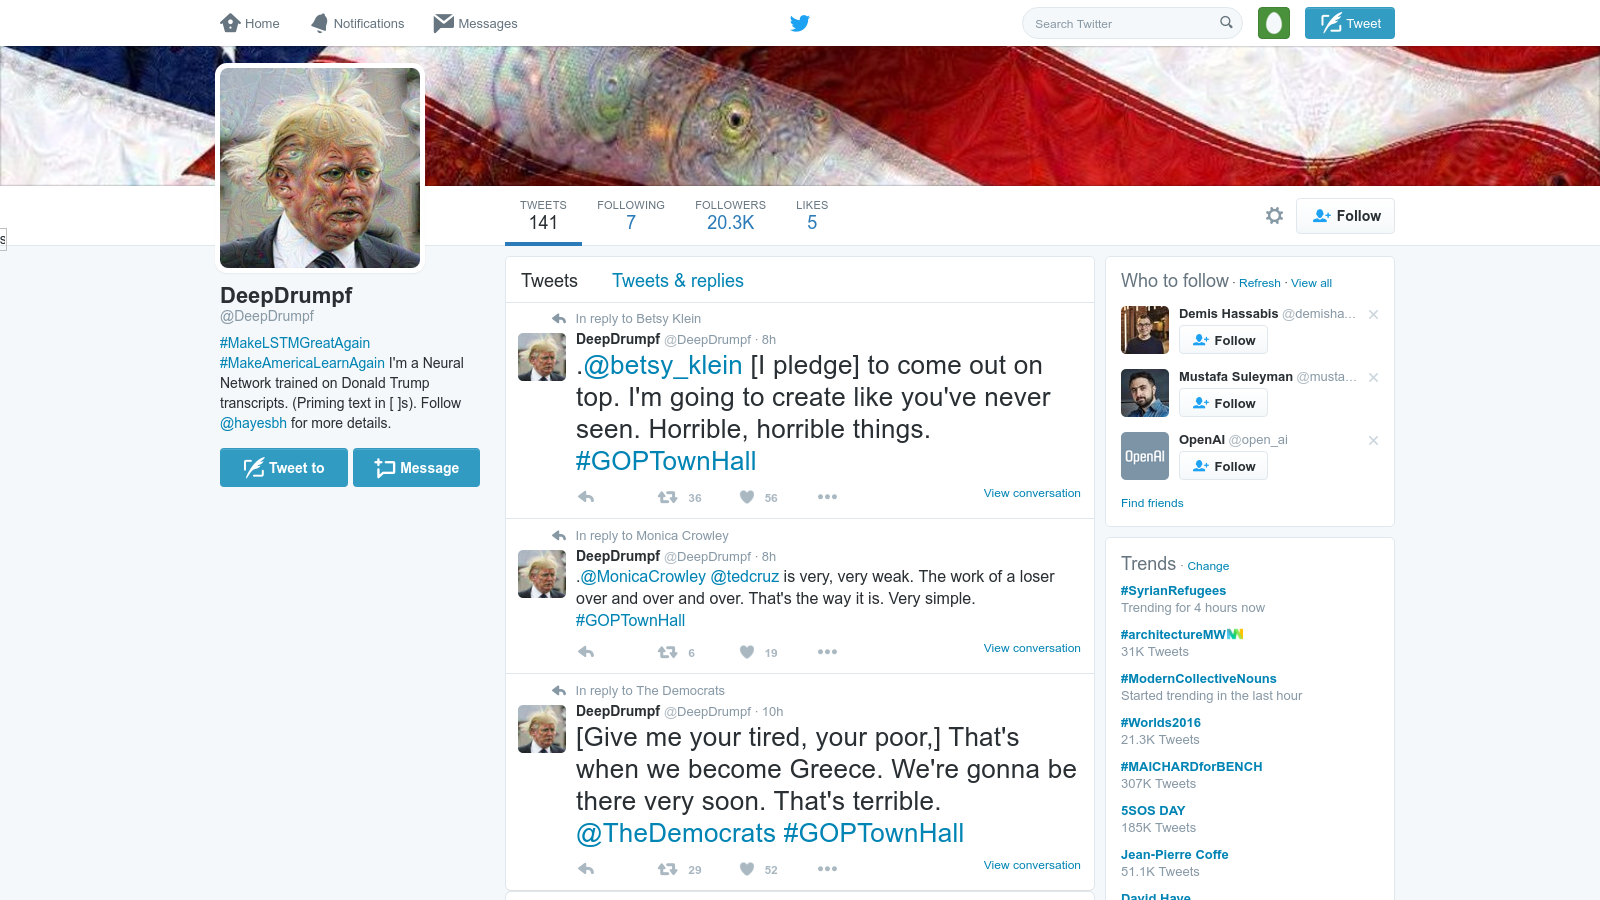
\includegraphics[width=\textwidth]{../img/DeepDrumpf.png}
    \end{frame}
  }

  {
    \setbeamertemplate{frame footer}{\cite{Mnih2015human}}
    \begin{frame}{Atari Player by Google DeepMind}
      \begin{center}
        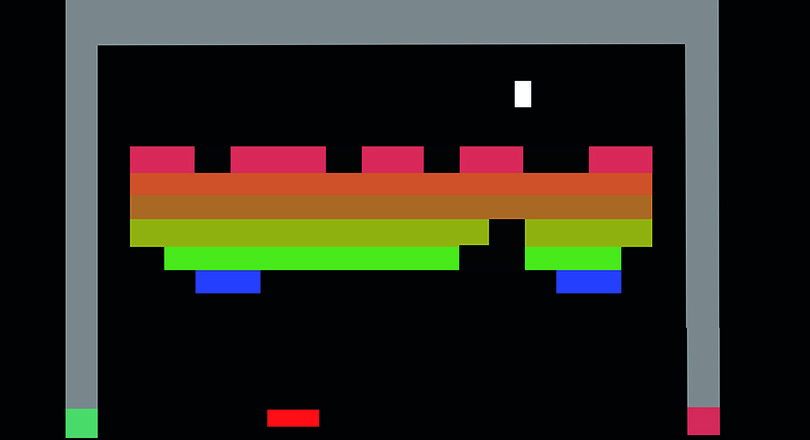
\includegraphics[width=\textwidth, height=\textheight, keepaspectratio]{../img/atari_breakout.jpg}

        \url{https://youtu.be/0X-NdPtFKq0?t=16m57s}
      \end{center}
    \end{frame}
  }

  \begin{frame}[standout]
    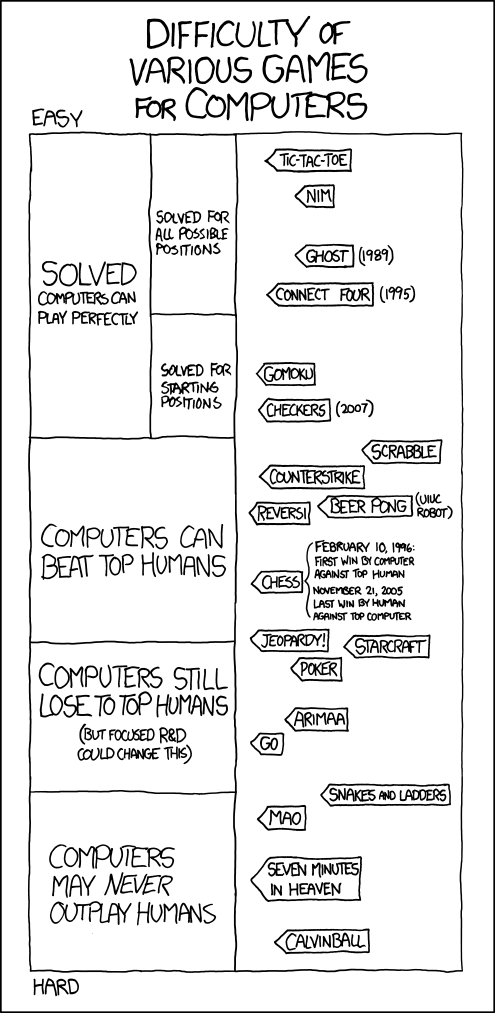
\includegraphics[height=\paperheight]{../img/game_AIs.png}
    \nocite{xkcdGameAIs}
  \end{frame}

  {
    \setbeamertemplate{frame footer}{\cite{Bowling2015heads}}
    \begin{frame}{Heads-up Limit Hold’em Poker Is Solved!}
      \pause
      \begin{center}
        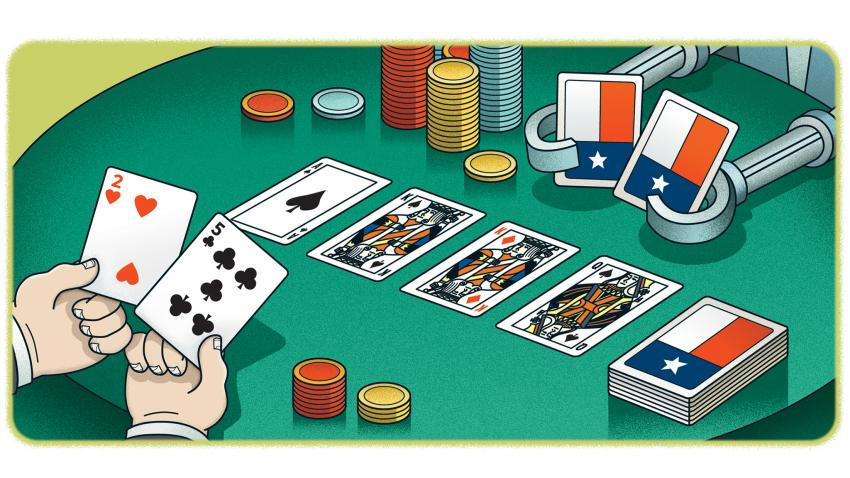
\includegraphics[width=\textwidth, keepaspectratio]{../img/limit_holdem_poker.jpg}

        \textbf{Cepheus} \url{http://poker.srv.ualberta.ca/}
      \end{center}
    \end{frame}
  }

%%%%%%%%%%%%%%%%%%%%%%%%%%%%%%%%%%%%%%%%%%%%%%%%%%%%%%%%%%%%%%%%%%%%%%%%%%%%%%%%

  \section{Basics of Machine learning}

  \begin{frame}{Supervised versus Unsupervised Learning}
    Supervised learning
    \begin{itemize}[<+- | alert@+>]
      \item \todo
      \item \todo
    \end{itemize}
    \pause

    Unsupervised learning:
    \begin{itemize}[<+- | alert@+>]
      \item \todo
      \item \todo
    \end{itemize}
  \end{frame}

  {
    \setbeamertemplate{frame footer}{\url{http://www.nickgillian.com/}}
    \begin{frame}{Supervised Learning}
      \begin{center}
        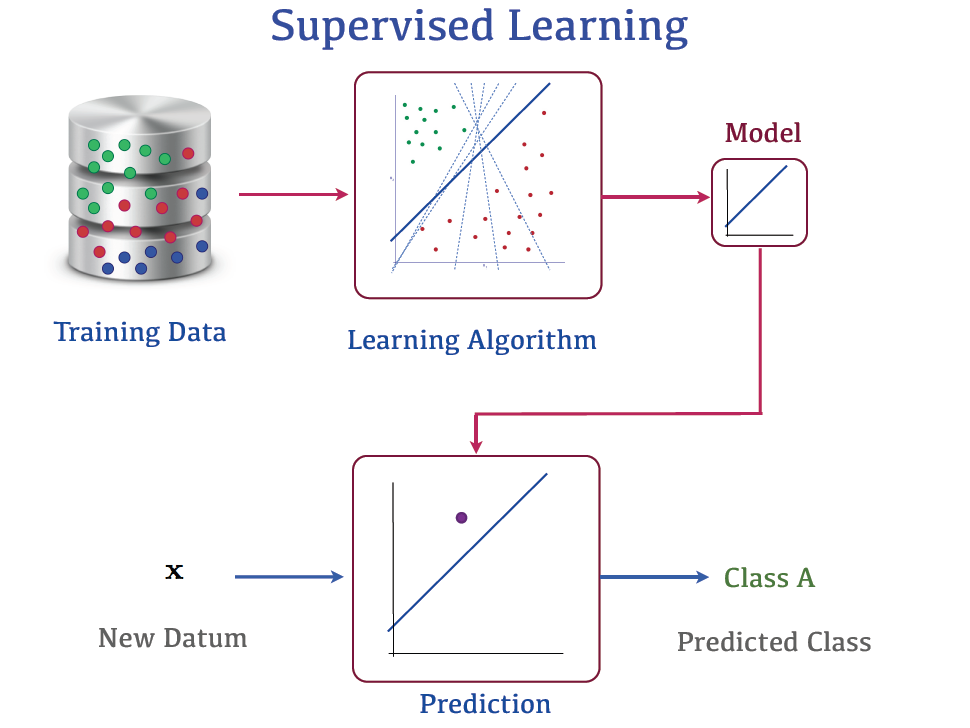
\includegraphics[height=.6\textheight]{../img/SL_workflow.png}
      \end{center}
      \pause

      \begin{enumerate}[<+- | alert@+>]
          \tiny
        \item data collection: Google Search, Facebook ``Likes'', Siri, Netflix, YouTube views, LHC collisions, \textbf{KGS Go Server}...
        \item training on~\textbf{training set}
        \item testing on~\textbf{testing set}
        \item deployment
      \end{enumerate}
      \pause
    \end{frame}
  }

  \begin{frame}{Regression}
    \pause
    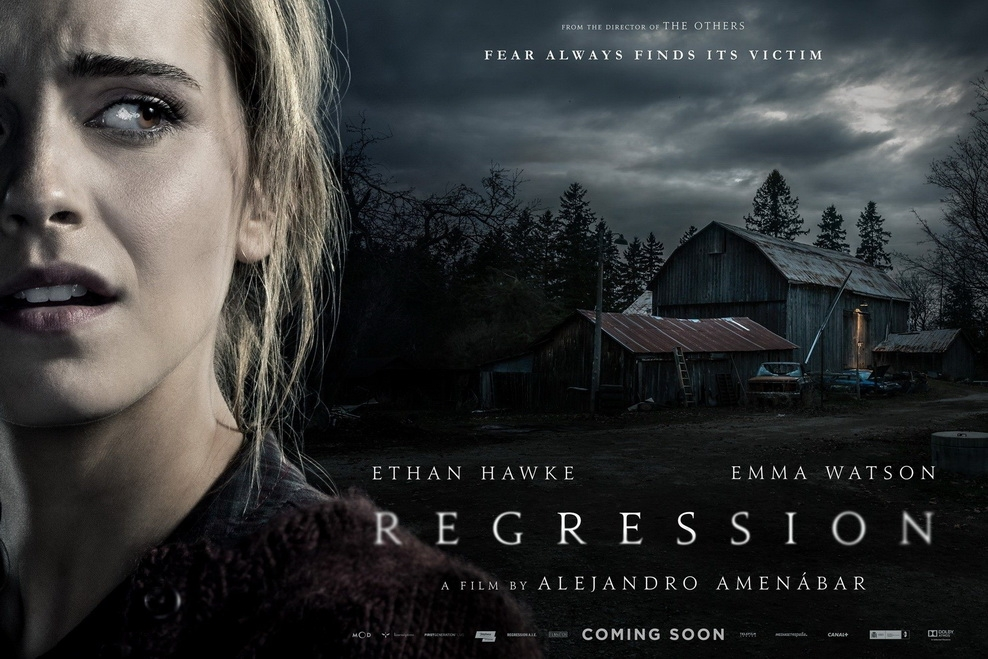
\includegraphics[width=\textwidth]{../img/regression_movie.jpg}
  \end{frame}

  {
    \setbeamertemplate{frame footer}{\url{https://thermanuals.wordpress.com/descriptive-analysis/sampling-and-regression/}}
    \begin{frame}{Mathematical Regression}
      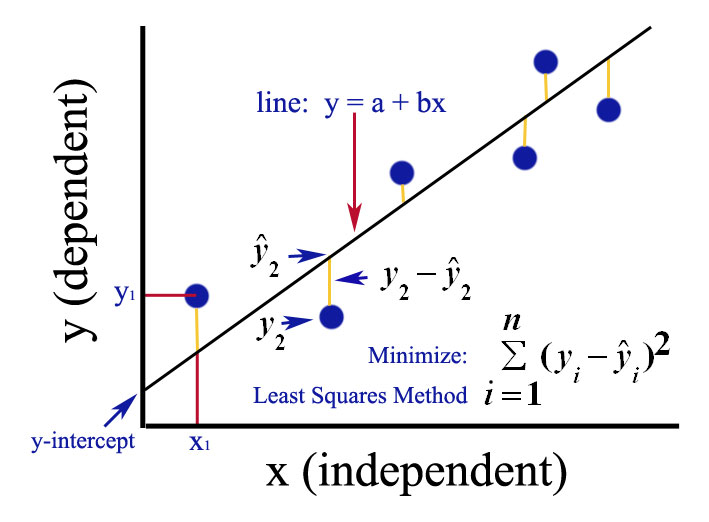
\includegraphics[width=\textwidth]{../img/regression_math.jpg}
    \end{frame}
  }

  {
    \setbeamertemplate{frame footer}{\url{https://kevinbinz.files.wordpress.com/2014/08/ml-svm-after-comparison.png}}
    \begin{frame}{Classification}
      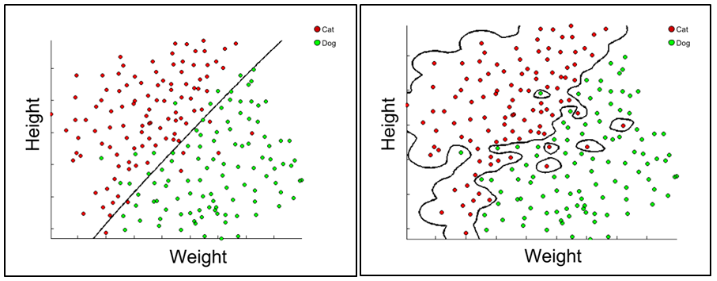
\includegraphics[width=\textwidth]{../img/classification.png}
    \end{frame}
  }

  {
    \setbeamertemplate{frame footer}{\url{https://www.researchgate.net/post/How_to_Avoid_Overfitting}}
    \begin{frame}{Underfitting and Overfitting}
      \begin{center}
        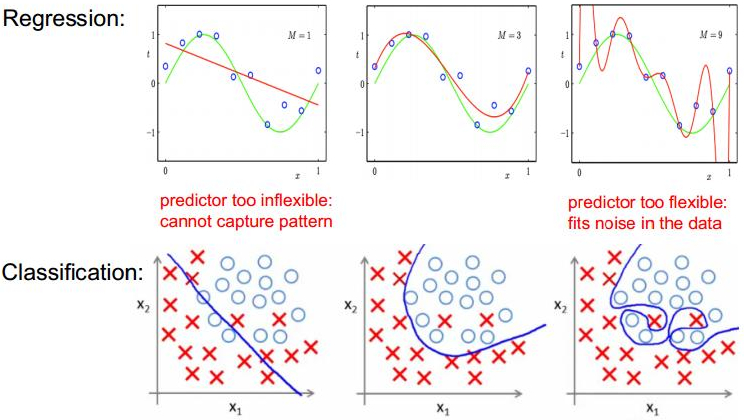
\includegraphics[width=.75\textwidth]{../img/underfitting_and_overfitting.jpg}
        \pause
      \end{center}

      Beware of~overfitting!
      \pause

      It is like learning for~a~mathematical exam by~memorizing proofs.
    \end{frame}
  }

  {
    \setbeamertemplate{frame footer}{\url{https://youtu.be/0X-NdPtFKq0?t=16m57s}}
    \begin{frame}{Reinforcement Learning}
      \begin{center}
        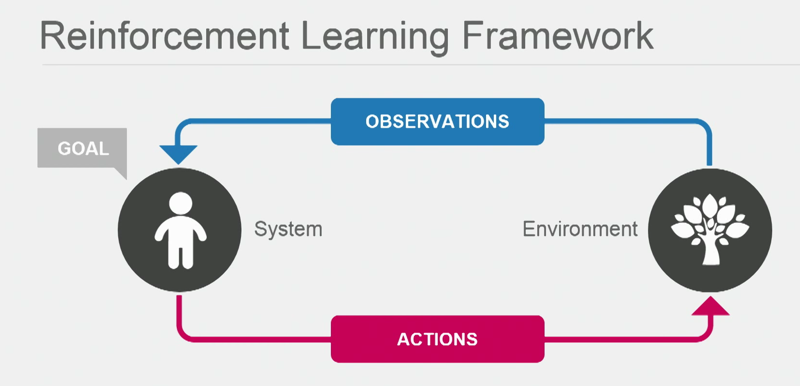
\includegraphics[width=\textwidth]{../img/RL_framework.png}
      \end{center}
      \pause
      
      Specially: games of \textbf{self-play}
    \end{frame}
  }

%%%%%%%%%%%%%%%%%%%%%%%%%%%%%%%%%%%%%%%%%%%%%%%%%%%%%%%%%%%%%%%%%%%%%%%%%%%%%%%%

  \section{Monte Carlo Tree Search}
  {
    \setbeamertemplate{frame footer}{\cite{Silver2016mastering}}
    \begin{frame}{Tree Search}
      Optimal value~$v^*(s)$ determines the~outcome of~the game:
      \pause
      \begin{itemize}[<+- | alert@+>]
          \tiny
        \item from every board position or state $s$
        \item under perfect play by~all players.
      \end{itemize}
      \pause

      It is computed by~\textbf{recursively traversing a~search tree} containing approximately $b^d$ possible sequences of moves, where
      \pause
      \begin{itemize}[<+- | alert@+>]
          \tiny
        \item $b$ is the game’s breadth (number of legal moves per position)
        \item $d$ is its depth (game length)
      \end{itemize}
    \end{frame}
  }

  {
    \setbeamertemplate{frame footer}{\cite{Allis1994searching}}
    \begin{frame}{Game tree of~Go}
      Sizes of~trees for~various games:
      \begin{itemize}
        \item chess: $b \approx 35, d \approx 80$
        \item Go: $b \approx 250, d \approx 150$
          \pause
          $\Rightarrow$ more positions than atoms in the universe!
      \end{itemize}
      \pause

      \epigraph{
        That makes Go a \textbf{googol} times more complex than chess.
      }{\tiny\url{https://deepmind.com/alpha-go.html}}
      \pause

      \vskip -1em
      How to handle the size~of the game tree?
      \pause
      \begin{itemize}[<+- | alert@+>]
        \item for the breadth: a~neural network to~select moves 
        \item for the depth: a~neural network to~evaluate current position
        \item for the tree traverse: Monte Carlo tree search (MCTS)
      \end{itemize}
    \end{frame}
  }

  \begin{frame}{Monte Carlo tree search}
    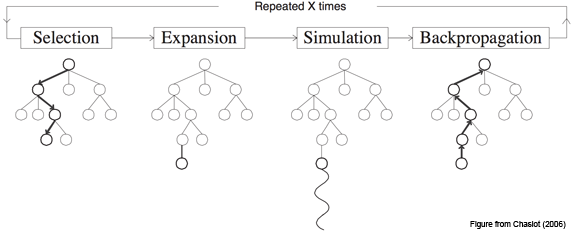
\includegraphics[width=\textwidth]{../img/MCTS.png}
  \end{frame}

%%%%%%%%%%%%%%%%%%%%%%%%%%%%%%%%%%%%%%%%%%%%%%%%%%%%%%%%%%%%%%%%%%%%%%%%%%%%%%%%

  \section{Neural networks}
  {
    \setbeamertemplate{frame footer}{\url{http://pages.cs.wisc.edu/~bolo/shipyard/neural/local.html}}
    \begin{frame}{Neural Network: Inspiration}
      \vskip -2em
      \begin{center}
        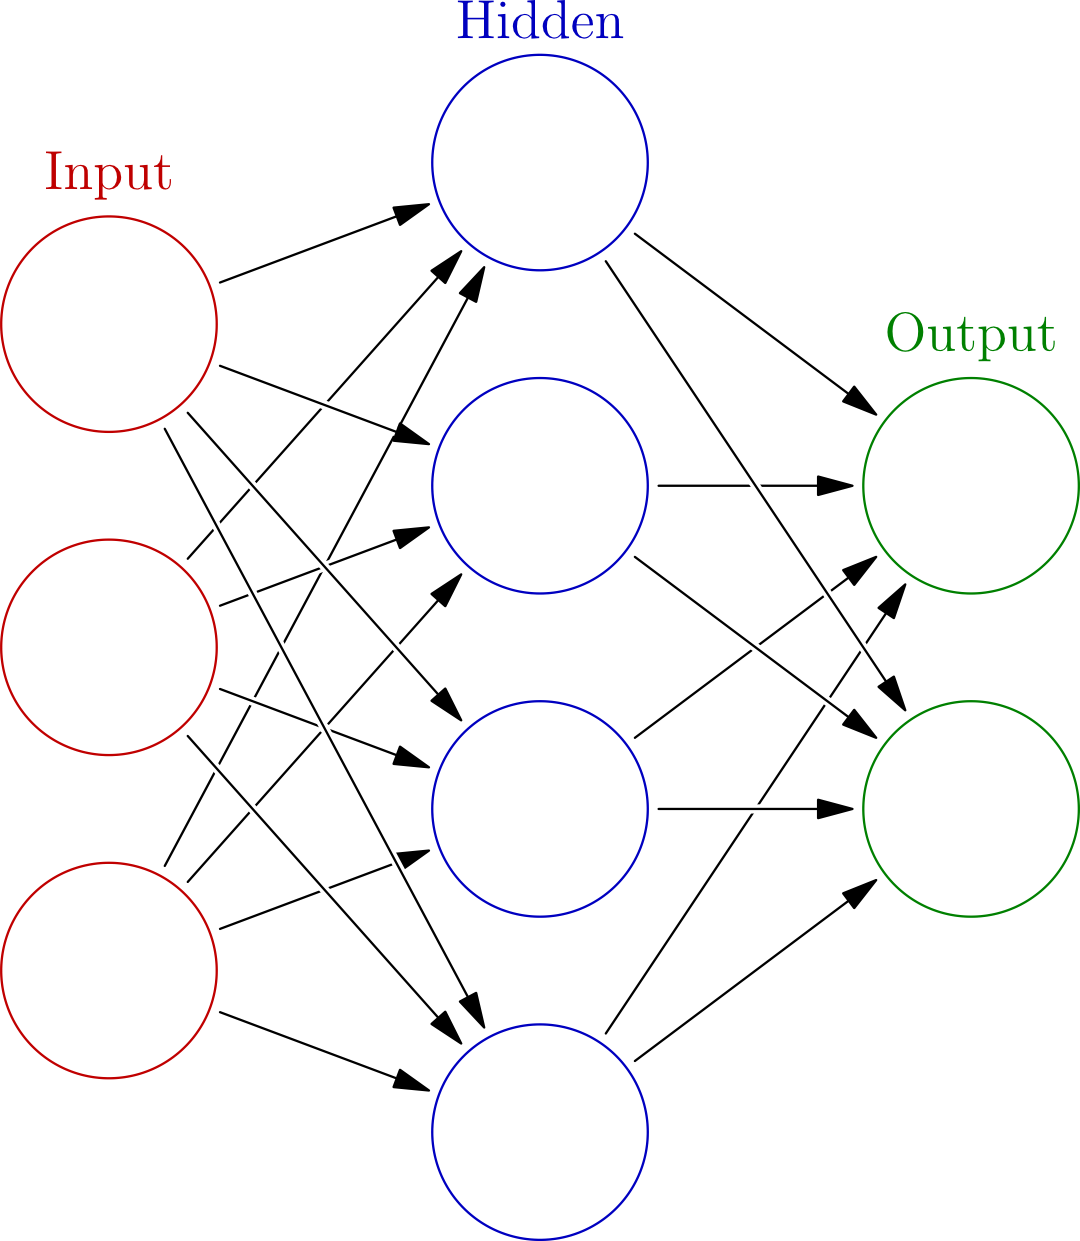
\includegraphics[height=.5\textheight]{../img/colored_neural_network.png}
      \end{center}

      \pause
      \begin{itemize}[<+- | alert@+>]
        \item inspired by~the neuronal structure of~the mammalian cerebral cortex
        \item but on~much smaller scales
        \item suitable to model systems with a~high tolerance to~error 
          \begin{itemize}
            \item e.g.~audio or~image recognition
          \end{itemize}
      \end{itemize}
    \end{frame}
  }

  {
    \setbeamertemplate{frame footer}{\cite{Dieterle2003multianalyte}}
    \begin{frame}{Neural Network: Modes}
      \begin{center}
        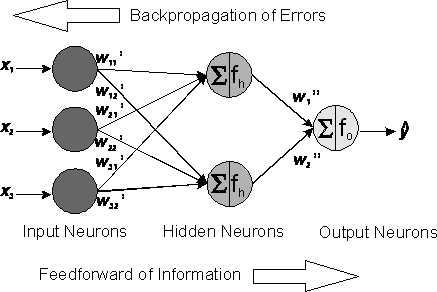
\includegraphics[height=.6\textheight]{../img/neural_network_forward_and_backprop.png}
      \end{center}

      \pause
      Two modes
      \pause
      \begin{itemize}[<+- | alert@+>]
        \item \textbf{feedforward} for making predictions
        \item \textbf{backpropagation} for learning
      \end{itemize}
    \end{frame}
  }

  {
    \setbeamercolor{background canvas}{bg=gray!10}
    \setbeamertemplate{frame footer}{\url{http://stevenmiller888.github.io/mind-how-to-build-a-neural-network/}}
    \begin{frame}{Neural Network: an~example of~feedforward}
      \begin{center}
        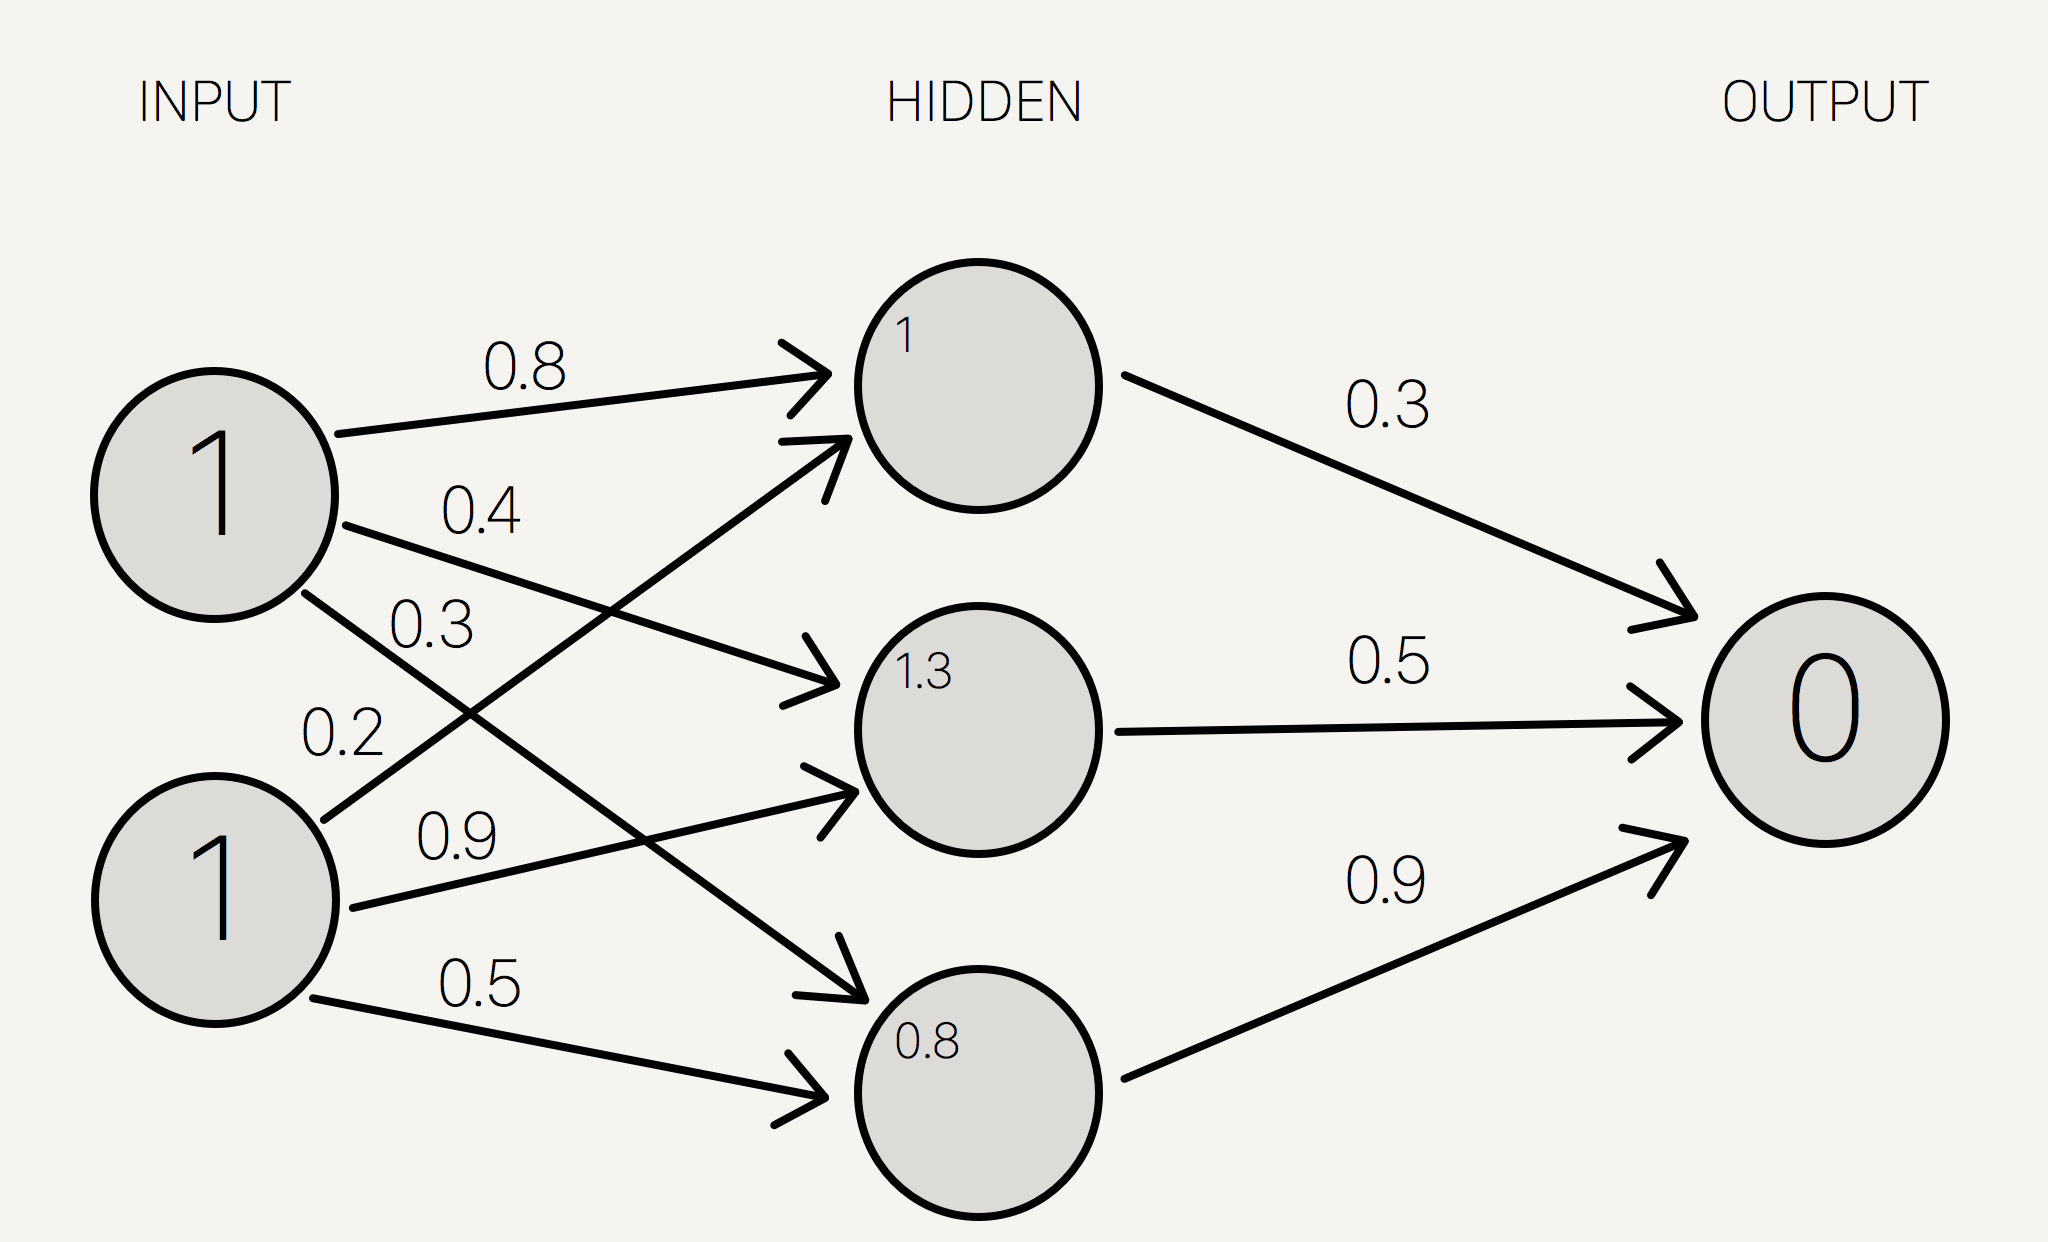
\includegraphics[width=\textwidth]{../img/feed_forward_example.png}
      \end{center}
    \end{frame}
  }

  {
    \setbeamertemplate{frame footer}{\url{http://pages.cs.wisc.edu/~bolo/shipyard/neural/local.html}}
    \begin{frame}{Gradient Descent in~Neural Networks}
      \pause
      Motto: "Learn by mistakes!"
      \begin{center}
        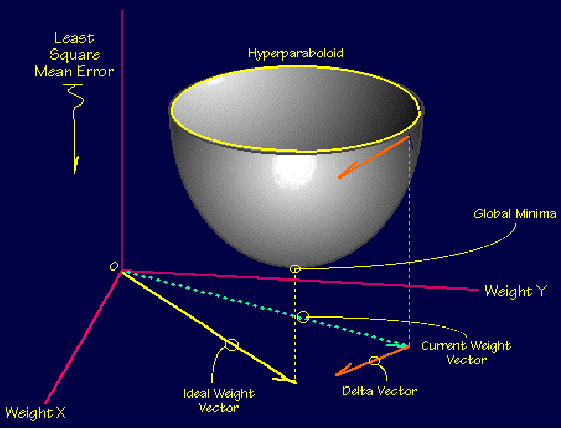
\includegraphics[height=.7\textheight]{../img/optimization_for_neural_networks.png}
      \end{center}
      \pause

      \vskip -1em
      However, error functions are not necessarily convex or~so ``smooth''.
    \end{frame}
  }

  {
    \setbeamertemplate{frame footer}{\url{http://pages.cs.wisc.edu/~bolo/shipyard/neural/local.html}}
    \begin{frame}{Deep Neural Network: Inspiration}
      \vskip -2em
      \begin{center}
        \tiny
        The hierarchy of~concepts is captured in~the~number of~layers (the~\textbf{deep} in~``\textbf{deep} learning'')
        \pause

        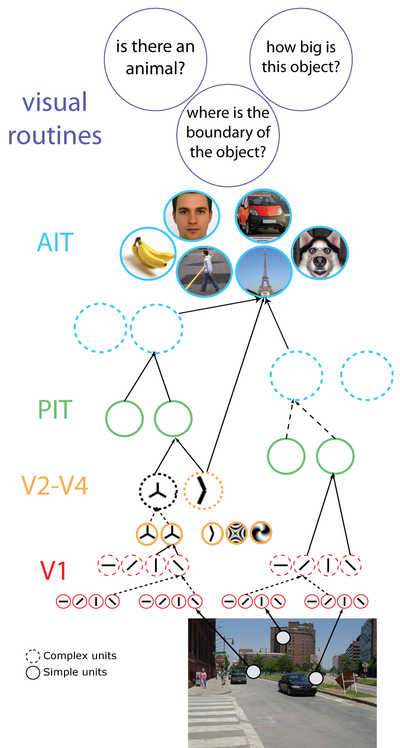
\includegraphics[height=.8\textheight]{../img/deep_learning_hierarchy.png}
      \end{center}
    \end{frame}

    \begin{frame}{Convolutional Neural Network}
      \begin{center}
        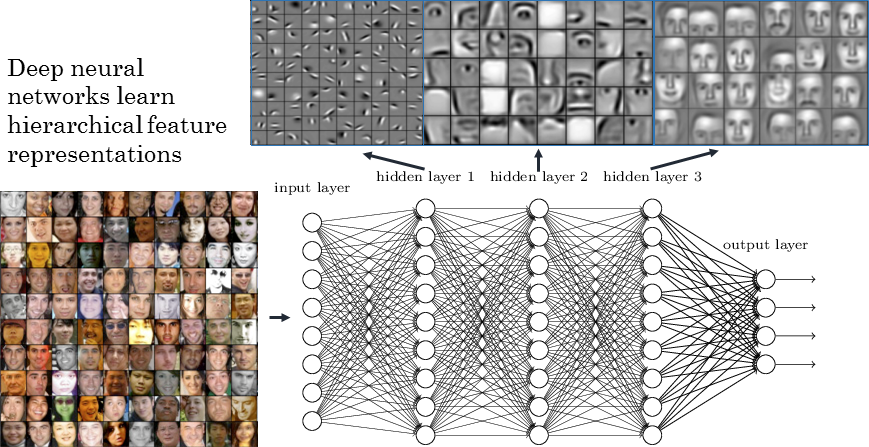
\includegraphics[width=\textwidth]{../img/ConvNet_hierarchy.png}
      \end{center}
    \end{frame}
  }

%%%%%%%%%%%%%%%%%%%%%%%%%%%%%%%%%%%%%%%%%%%%%%%%%%%%%%%%%%%%%%%%%%%%%%%%%%%%%%%%

  \section{Rules of Go}
  \begin{frame}{Classic games (1/2)}
    \pause
    \begin{center}
      \tiny
      Backgammon: Man vs. Fate

      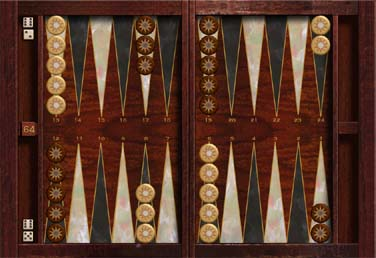
\includegraphics[height=.4\textheight]{../img/backgammon.jpg}
      \pause

      Chess: Man vs. Man

      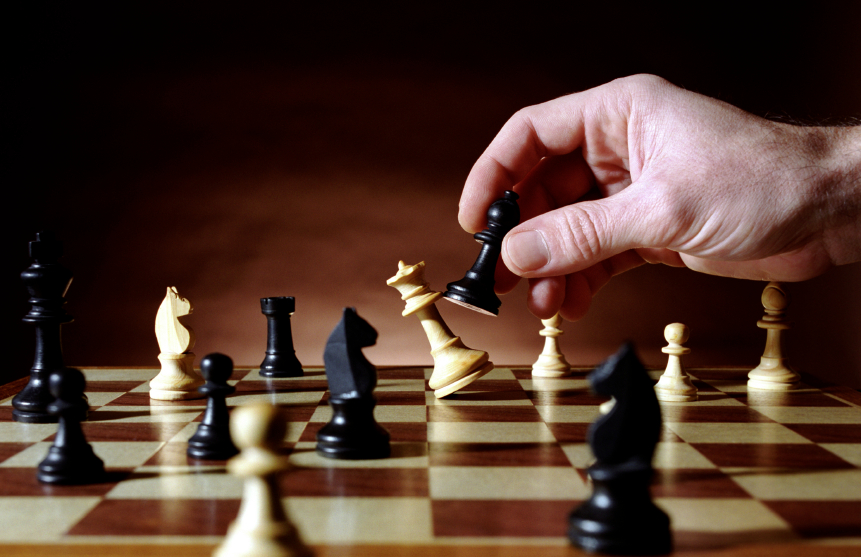
\includegraphics[height=.4\textheight]{../img/chess.jpg}
    \end{center}
  \end{frame}

  \begin{frame}{Classic games (2/2)}
    \begin{center}
      Go: Man vs. Self

      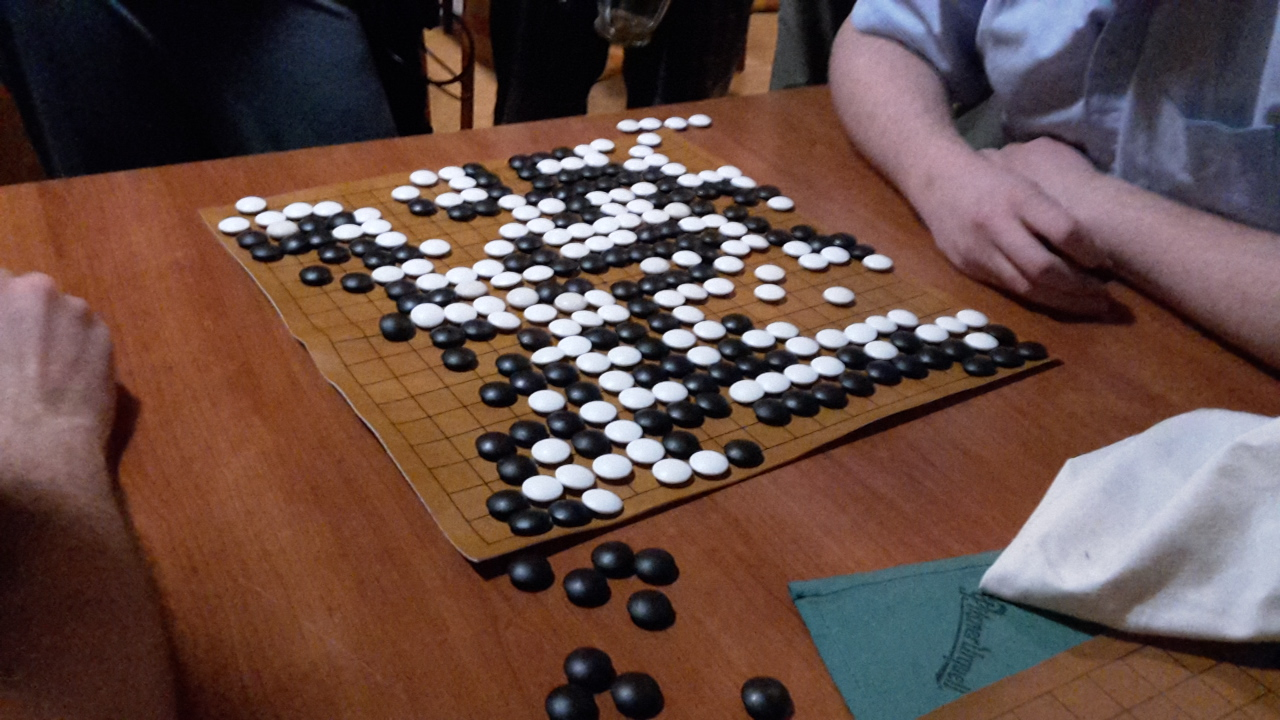
\includegraphics[width=.9\textwidth]{../img/Go_Samal_vs_Kral.jpg}
    \end{center}
  \end{frame}

  \begin{frame}{Rules of Go}
    \pause
    \textbf{Black} versus \textbf{White}.
    Black starts the game.
    \pause

    \pause
    \begin{center}
      \tiny
      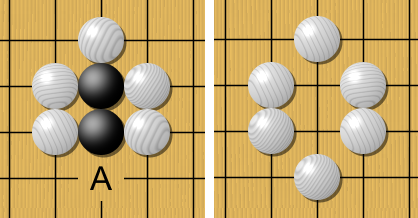
\includegraphics[width=.5\textwidth]{../img/Go_rule_of_liberty.png}

      the rule of liberty
      \pause


      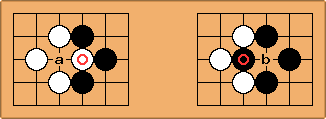
\includegraphics[width=.5\textwidth]{../img/Go_ko_rule.png}

      the ``ko'' rule
    \end{center}

    \pause
    \vskip -1em
    \textbf{Handicap} for difference in ranks:
    Black can place 1 or more stones in advance (compensation for White's greater strength).
  \end{frame}

  {
    \setbeamertemplate{frame footer}{\url{https://en.wikipedia.org/wiki/Go_(game)}}
    \begin{frame}{Scoring Rules: Area Scoring}
      \pause
      A player's score is:
      \begin{itemize}[<+- | alert@+>]
        \item the number of stones that the player has on the board
        \item plus the number of~empty intersections surrounded by that player's stones
        \item plus \textbf{komi(dashi)} points for the White player \\
          {\tiny which is a~compensation for the first move advantage of~the Black player}
      \end{itemize}
    \end{frame}

    \begin{frame}{Ranks of~Players}
      \begin{center}
        \tiny
        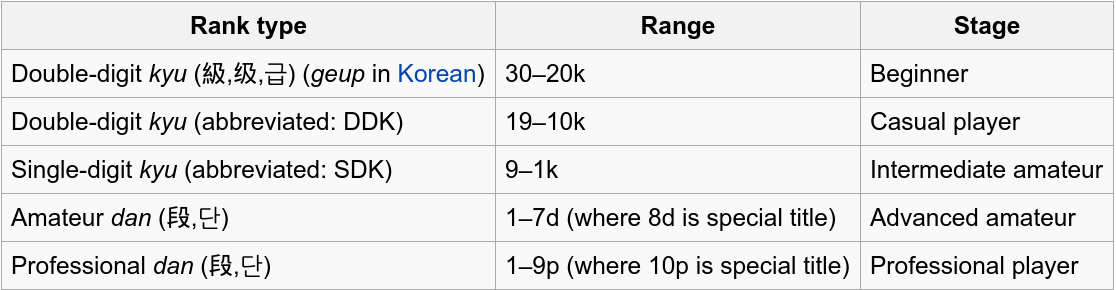
\includegraphics[width=\textwidth]{../img/Go_kyu_dan.png}

        \textbf{Kyu and Dan ranks}
      \end{center}
      \pause
      
      or alternatively, \textbf{ELO ratings}
    \end{frame}
  }

  {
    \usebackgroundtemplate{
      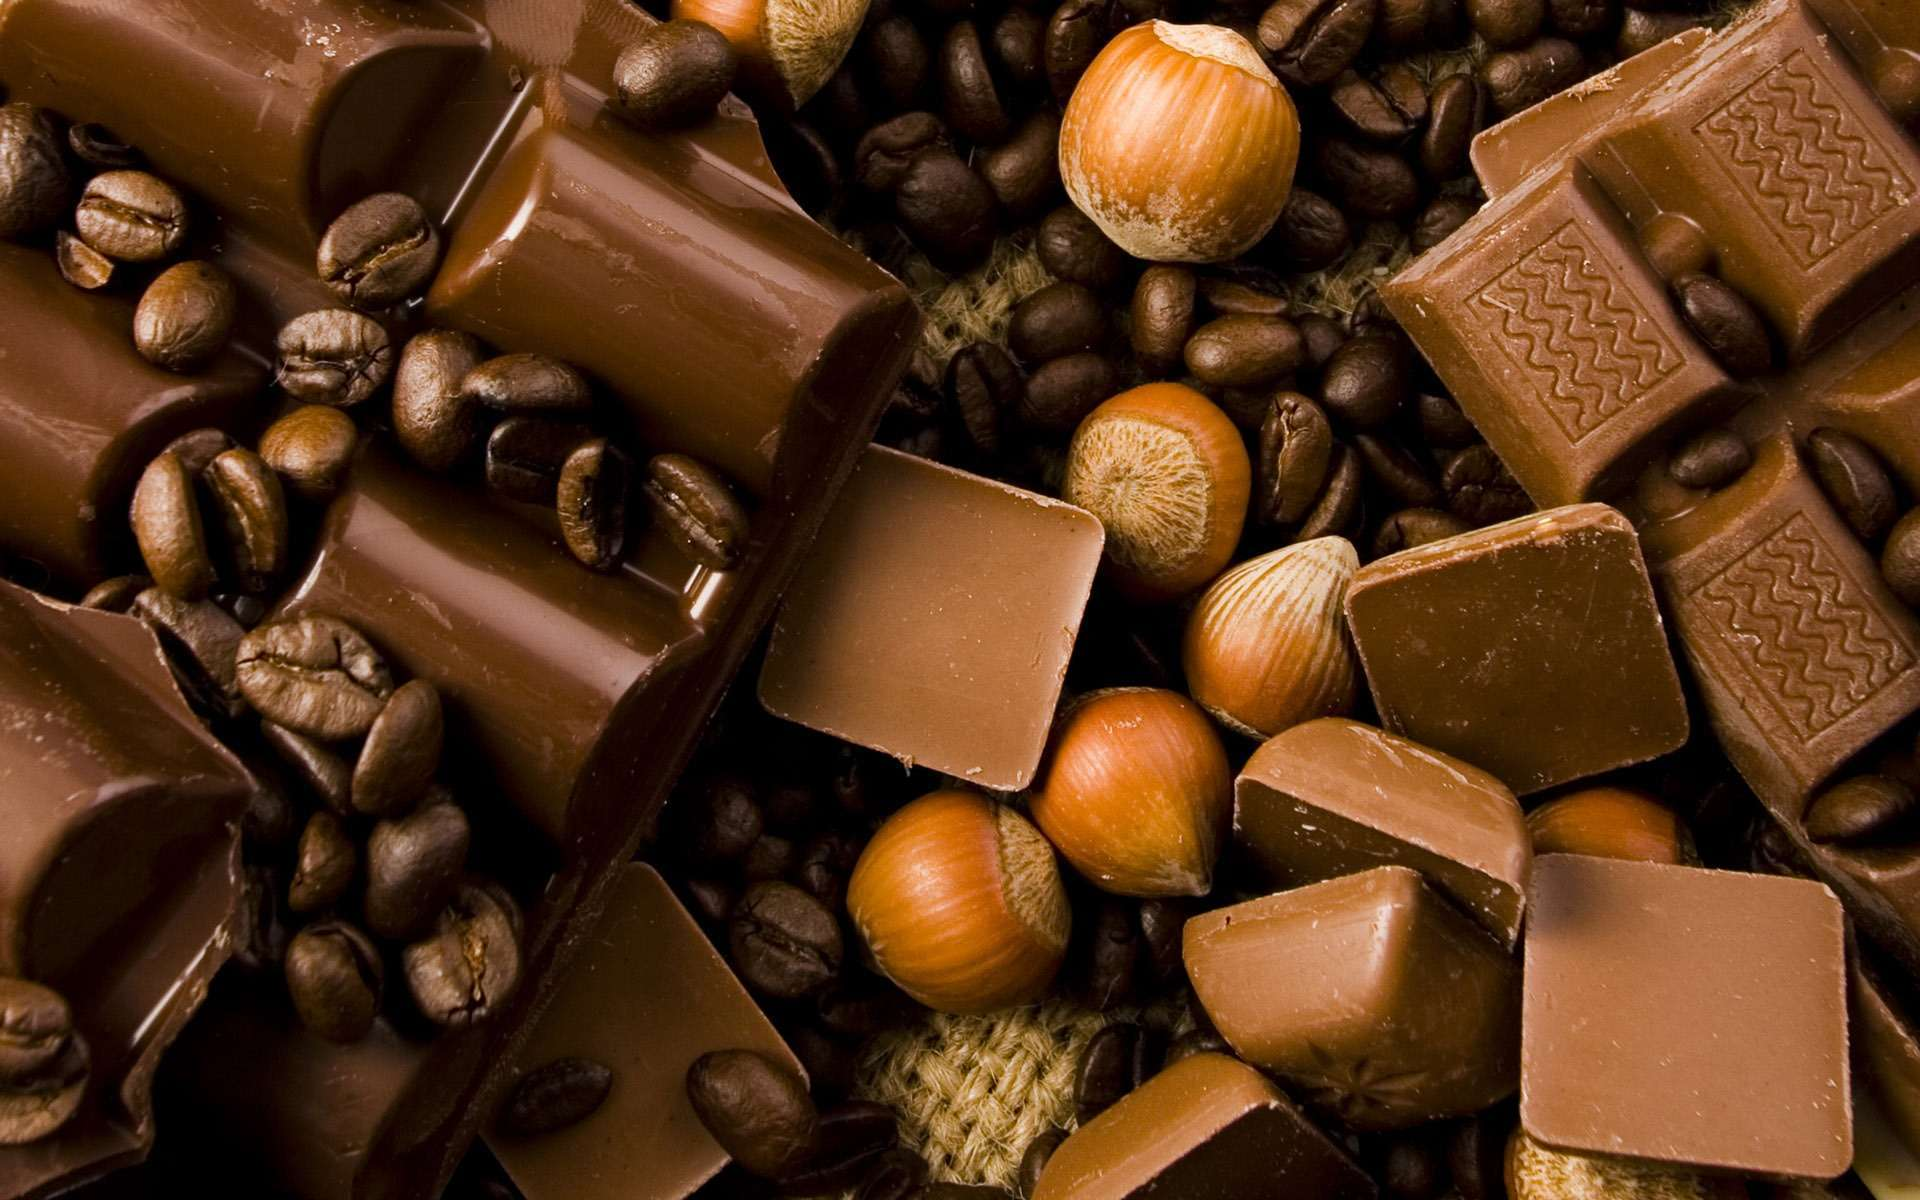
\includegraphics[height=\paperheight]{../img/swiss_choco.jpg}
    }
    \begin{frame}[standout, noframenumbering]
      Chocolate micro-break
    \end{frame}
  }

%%%%%%%%%%%%%%%%%%%%%%%%%%%%%%%%%%%%%%%%%%%%%%%%%%%%%%%%%%%%%%%%%%%%%%%%%%%%%%%%

  \section{AlphaGo: Inside Out}
  {
    \setbeamertemplate{frame footer}{\cite{Silver2016mastering}}
    \begin{frame}{Policy and Value Networks}
      \begin{center}
        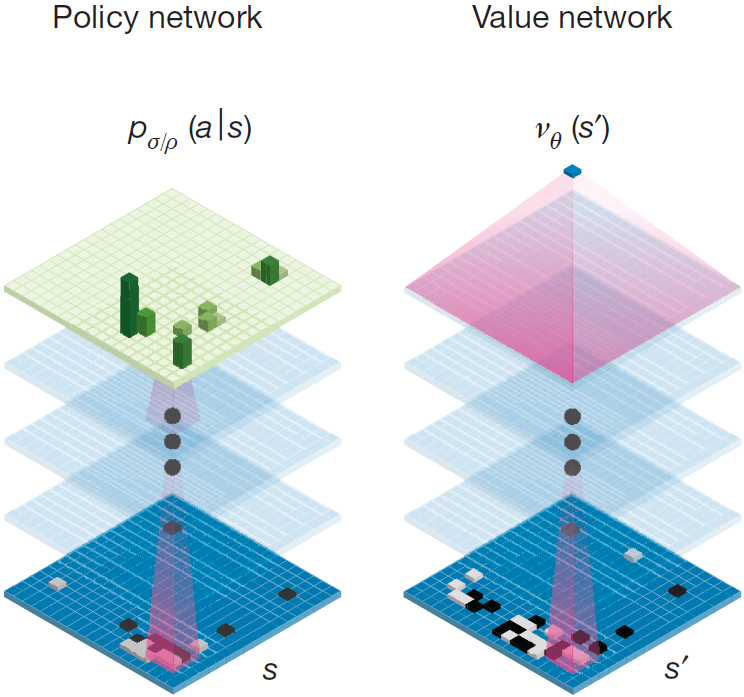
\includegraphics[height=.85\textheight]{../img/policy_and_value_network.png}
      \end{center}
    \end{frame}

    \begin{frame}{Training the (Deep Convolutional) Neural Networks}
      \begin{center}
        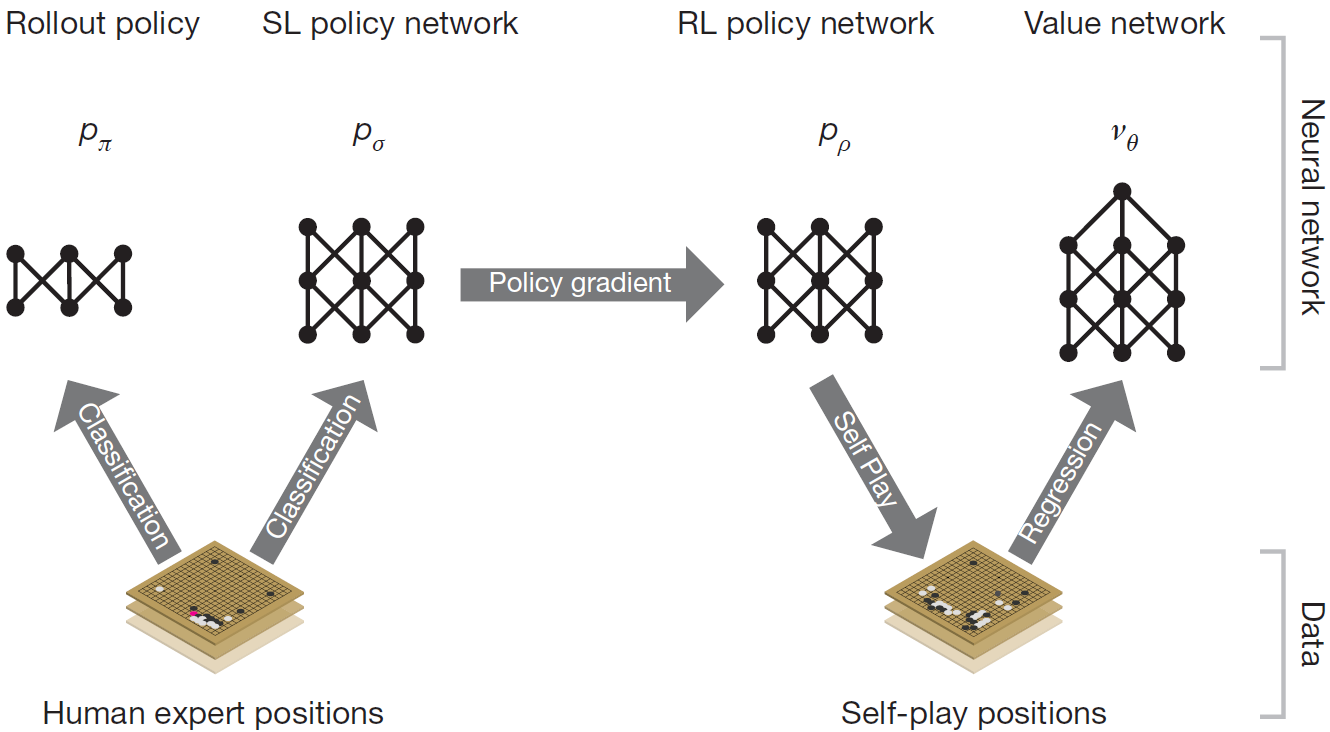
\includegraphics[width=\textwidth]{../img/neural_nets_pipeline.png}
      \end{center}
    \end{frame}

    \begin{frame}{SL Policy Networks (1/3)}
      \begin{itemize}[<+- | alert@+>]
        \item 13-layer deep convolutional neural network
        \item goal: to~predict expert human moves
        \item task of \textbf{classification}
        \item trained from 30 millions positions from the KGS Go Server
        \item stochastic gradient ascent:
          \[
            \Delta \sigma \propto \frac{\partial \log p_\sigma (a|s)}{\partial \sigma}
          \]
          {\tiny (to~maximize the likelihood of~the human move~$a$ selected in~state~$s$)}
      \end{itemize}
      \pause

      Results:
      \pause
      \begin{itemize}[<+- | alert@+>]
        \item $44.4\%$ accuracy (the state-of-the-art from other groups)
        \item $55.7\%$ accuracy (raw board position + move history as~input)
        \item $57.0\%$ accuracy (all input features)
      \end{itemize}
    \end{frame}

    \begin{frame}{SL Policy Networks (2/3)}
      Small improvements in~accuracy led to~large improvements in~playing strength (see the next slide)
      \begin{center}
        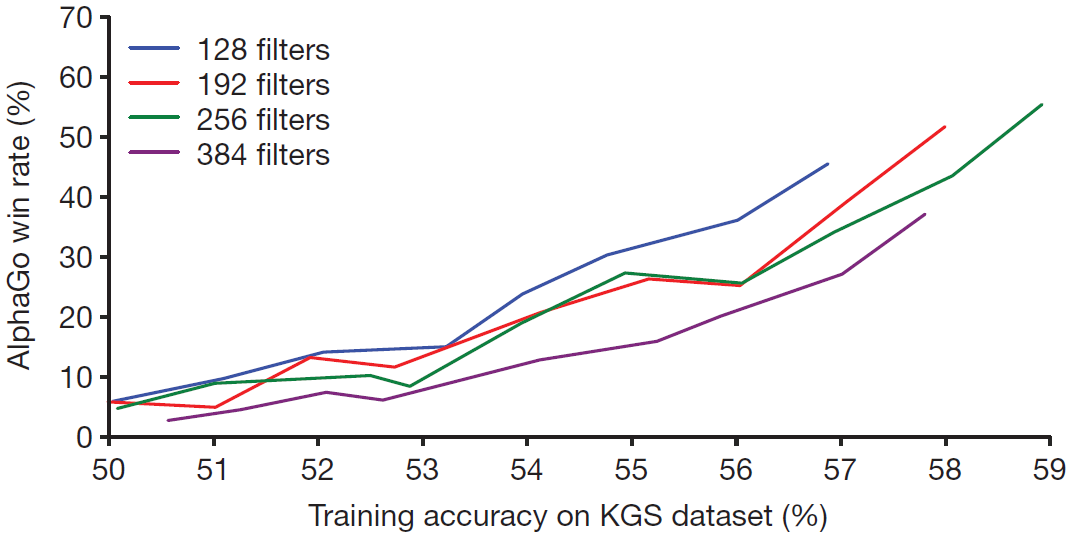
\includegraphics[width=\textwidth]{../img/SL_policy_accuracy_vs_win_rate.png}
      \end{center}
    \end{frame}

    \begin{frame}{SL Policy Networks (3/3)}
      \begin{center}
        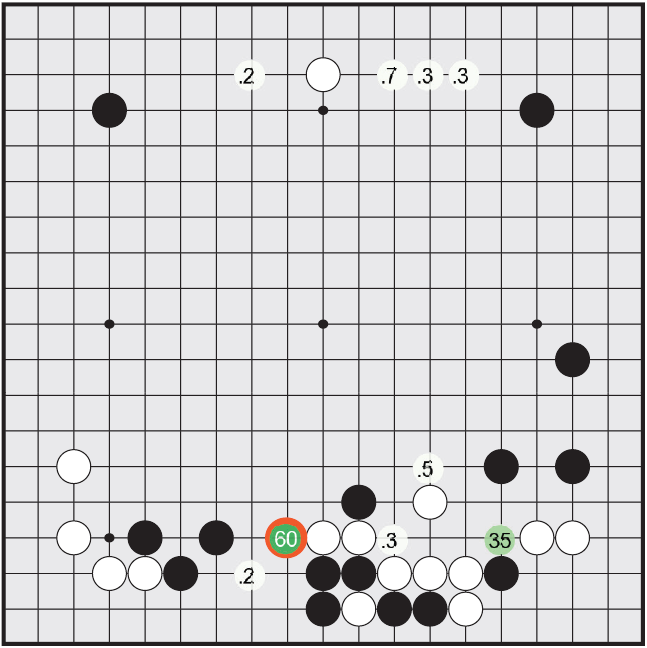
\includegraphics[height=.8\textheight]{../img/eval_SL_policy_network.png}

        \tiny
        move probabilities taken directly from the SL policy network $p_\sigma$ (reported as a~percentage if above $0.1\%$).
      \end{center}
    \end{frame}

    \begin{frame}{Training the (Deep Convolutional) Neural Networks}
      \begin{center}
        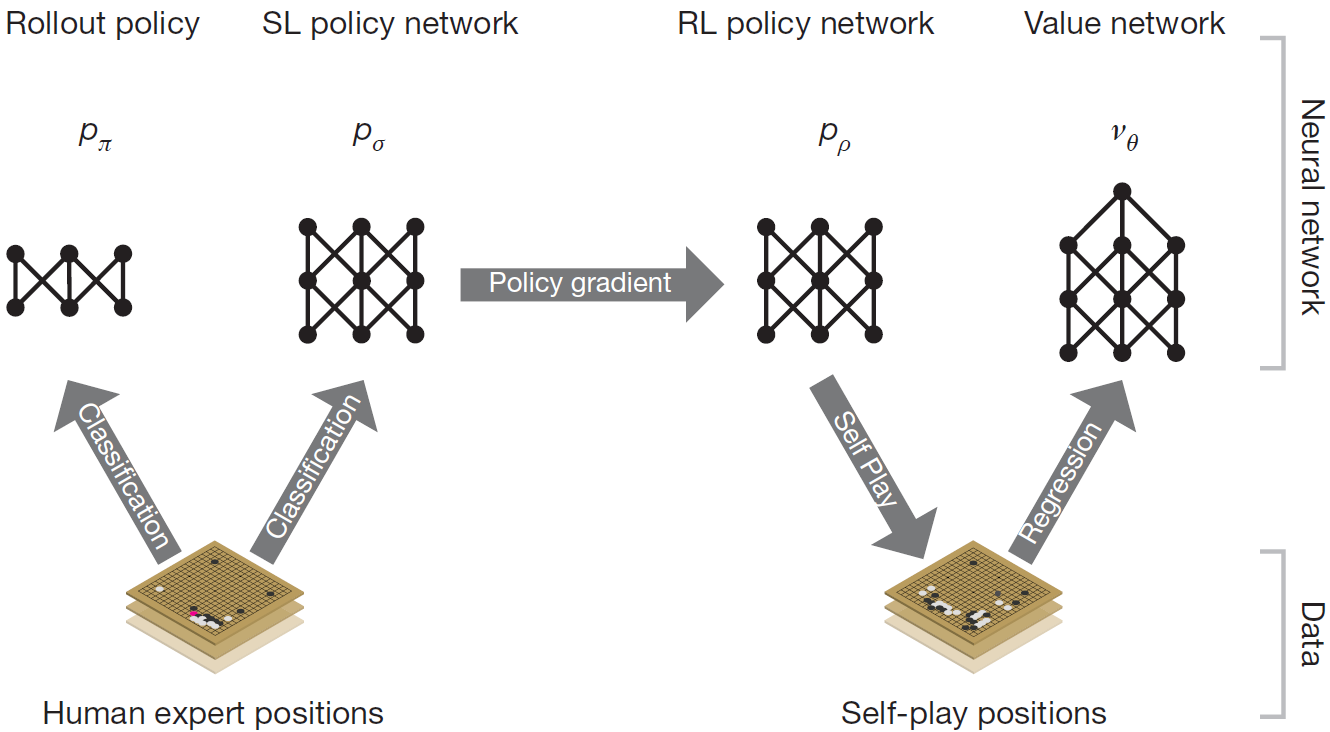
\includegraphics[width=\textwidth]{../img/neural_nets_pipeline.png}
      \end{center}
    \end{frame}

    \begin{frame}{Rollout Policy}
      \begin{itemize}[<+- | alert@+>]
        \item Rollout policy~$p_\pi(a|s)$ is \textbf{faster} but \textbf{less accurate} than SL policy network.
        \item accuracy of~$24.2\%$
        \item It takes $2 \mu$s to~select an~action, compared to $3$~ms in~case of~SL policy network.
      \end{itemize}
    \end{frame}

    \begin{frame}{Training the (Deep Convolutional) Neural Networks}
      \begin{center}
        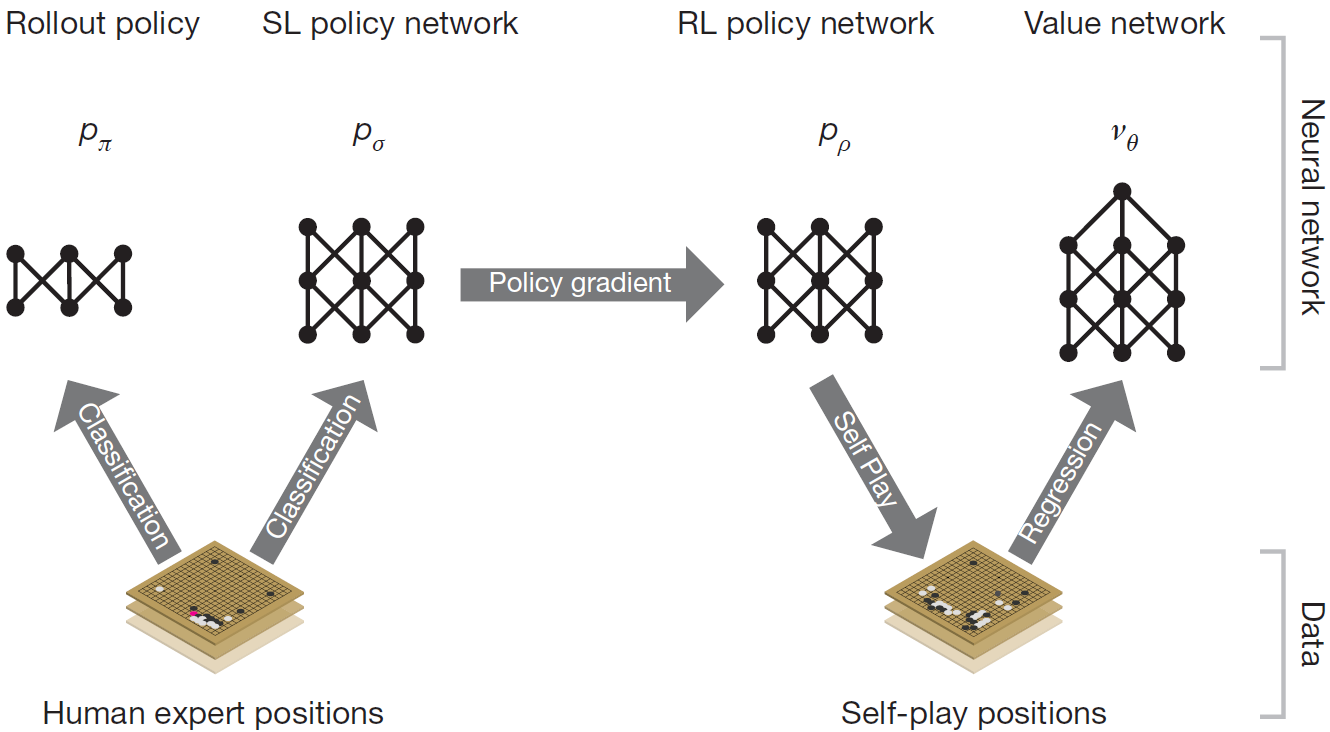
\includegraphics[width=\textwidth]{../img/neural_nets_pipeline.png}
      \end{center}
    \end{frame}

    \begin{frame}{RL Policy Networks (1/2)}
      \begin{itemize}[<+- | alert@+>]
        \item identical in~structure to the SL policy network
        \item goal: to~win in~the games of~self-play
        \item task of \textbf{classification}
        \item weights $\rho$ initialized to the same values, $\rho := \sigma$
        \item games of self-play
          \begin{itemize}[<+- | alert@+>]
            \item between the current RL policy network and a~randomly selected previous iteration
            \item to prevent overfitting to~the current policy
          \end{itemize}
        \item stochastic gradient ascent:
          \[
            \Delta \rho \propto \frac{\partial \log p_\rho (a_t|s_t)}{\partial \rho} z_t
          \]
          {\tiny at~time step~$t$, where reward function~$z_t$ is $+1$ for winning and $-1$ for losing.}
      \end{itemize}
      \pause
    \end{frame}

    \begin{frame}{RL Policy Networks (2/2)}
      Results (by sampling each move $a_t \sim p_\rho(\cdot | s_t)$):
      \pause
      \begin{itemize}[<+- | alert@+>]
        \item $80\%$ of~win rate against the SL policy network
        \item $85\%$ of~win rate against the strongest open-source Go program, \textbf{Pachi} (\cite{Baudivs2011pachi})
          \begin{itemize}[<+- | alert@+>]
            \item The previous state-of-the-art, based only on~SL of~CNN: \\
              \pause
              $11\%$ of~``win'' rate against Pachi
          \end{itemize}
      \end{itemize}
    \end{frame}

    \begin{frame}{Training the (Deep Convolutional) Neural Networks}
      \begin{center}
        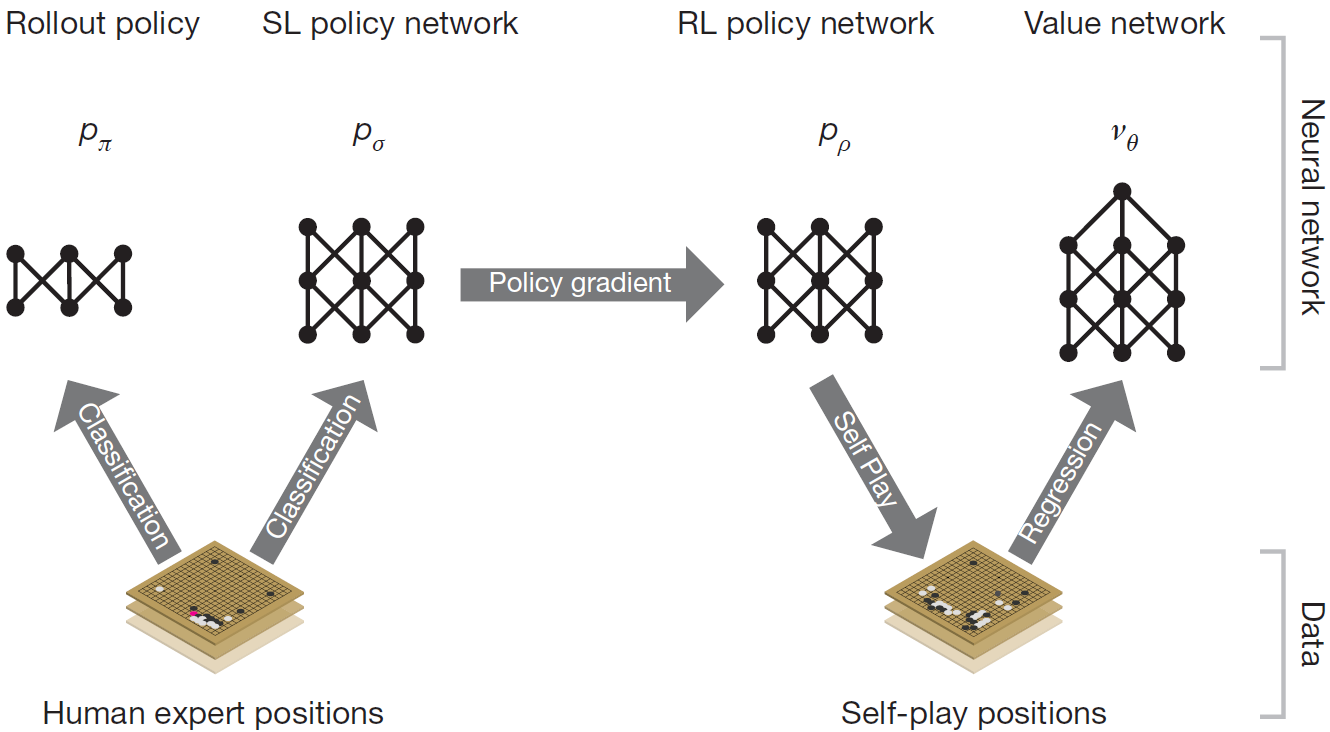
\includegraphics[width=\textwidth]{../img/neural_nets_pipeline.png}
      \end{center}
    \end{frame}

    \begin{frame}{Value Network (1/2)}
      \begin{itemize}[<+- | alert@+>]
        \item similar architecture to the policy network, but outputs a~single prediction instead of~a~probability distribution
        \item goal: to estimate a~value function
          \[
            v^p(s) = \E [z_t | s_t = s, a_{t \dots T} \sim p]
          \]
          that predicts the outcome from position~$s$ (of~games played by~using policy $p_\rho$)
        \item Specifically, $v_\theta(s) \approx v^{p_\rho}(s) \approx v^*(s)$.
        \item task of~\textbf{regression}
        \item stochastic gradient descent:
          \[
            \Delta \theta \propto \frac{\partial v_\theta (s)}{\partial \theta} (z - v_\theta(s))
          \]
          {\tiny (to~minimize the mean squared error (MSE) between the predicted $v_\theta(s)$ and the true $z$)}
      \end{itemize}
    \end{frame}

    \begin{frame}{Value Network (2/2)}
      Beware of~overfitting!
      \pause
      \begin{itemize}[<+- | alert@+>]
        \item Successive positions are strongly correlated.
        \item Value network memorized the game outcomes, rather than generalizing to new positions.
        \item Solution: generate 30 million (new) positions, each sampled from a~\textbf{seperate} game
        \item almost the accuracy of~Monte Carlo rollouts (using $p_\rho$), but $15000$ times less computation!
      \end{itemize}
    \end{frame}

    \begin{frame}{Selection of~Moves by the Value Network}
      \begin{center}
        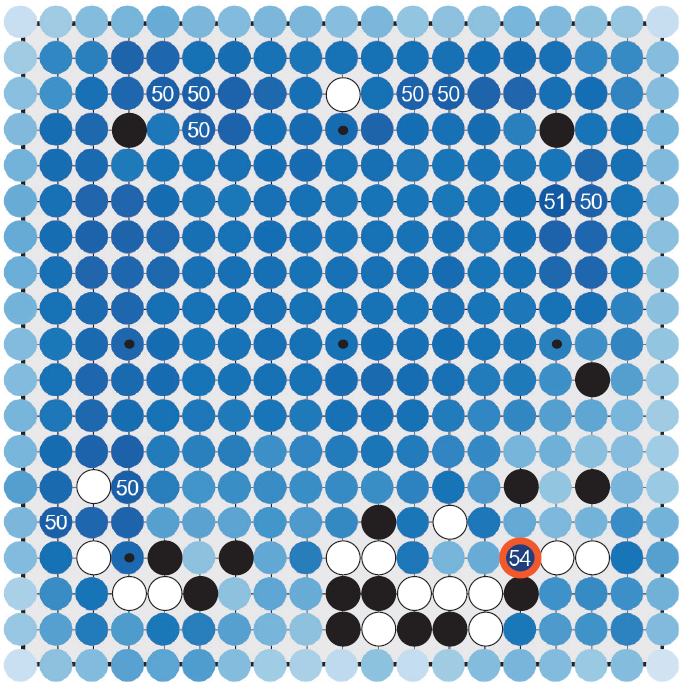
\includegraphics[height=.8\textheight]{../img/move_selection_by_value_network.png}

        \tiny
        evaluation of~all successors $s'$ of~the root position~$s$, using~$v_\theta(s′)$
      \end{center}
    \end{frame}

    \begin{frame}{Evaluation accuracy in~various stages of a~game}
      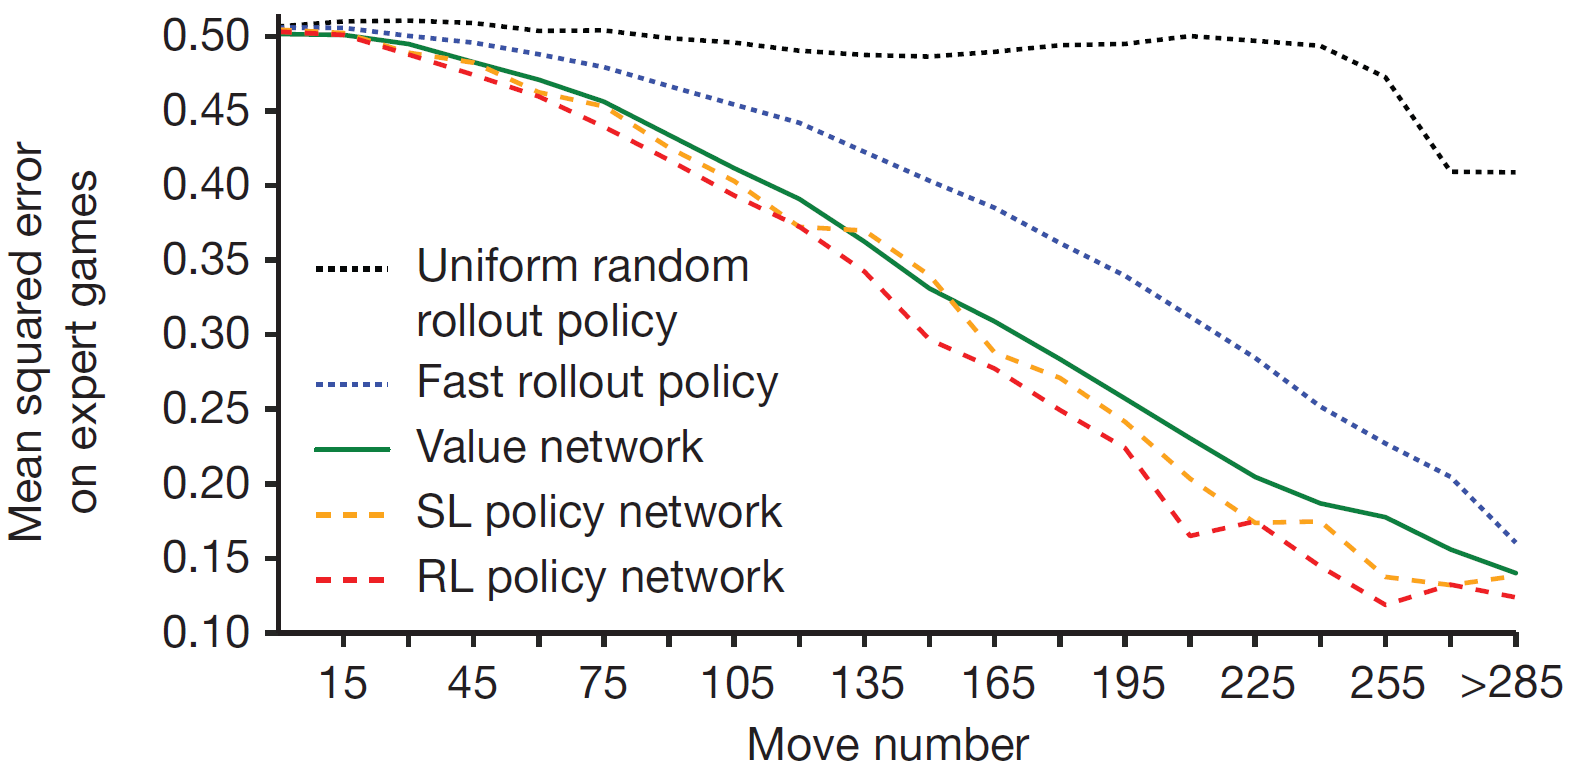
\includegraphics[width=\textwidth]{../img/policies_move_numbers_vs_MSE.png}

      \vskip -2.4ex
      {\tiny
      \textbf{Move number} is the number of~moves that had been played in the given position.
      }

      \pause
      Each position evaluated by:
      \begin{itemize}[<+- | alert@+>]
        \item forward pass of the value network~$v_\theta$
        \item 100 rollouts, played out using the corresponding policy
      \end{itemize}
    \end{frame}

    \begin{frame}{Training the (Deep Convolutional) Neural Networks}
      \begin{center}
        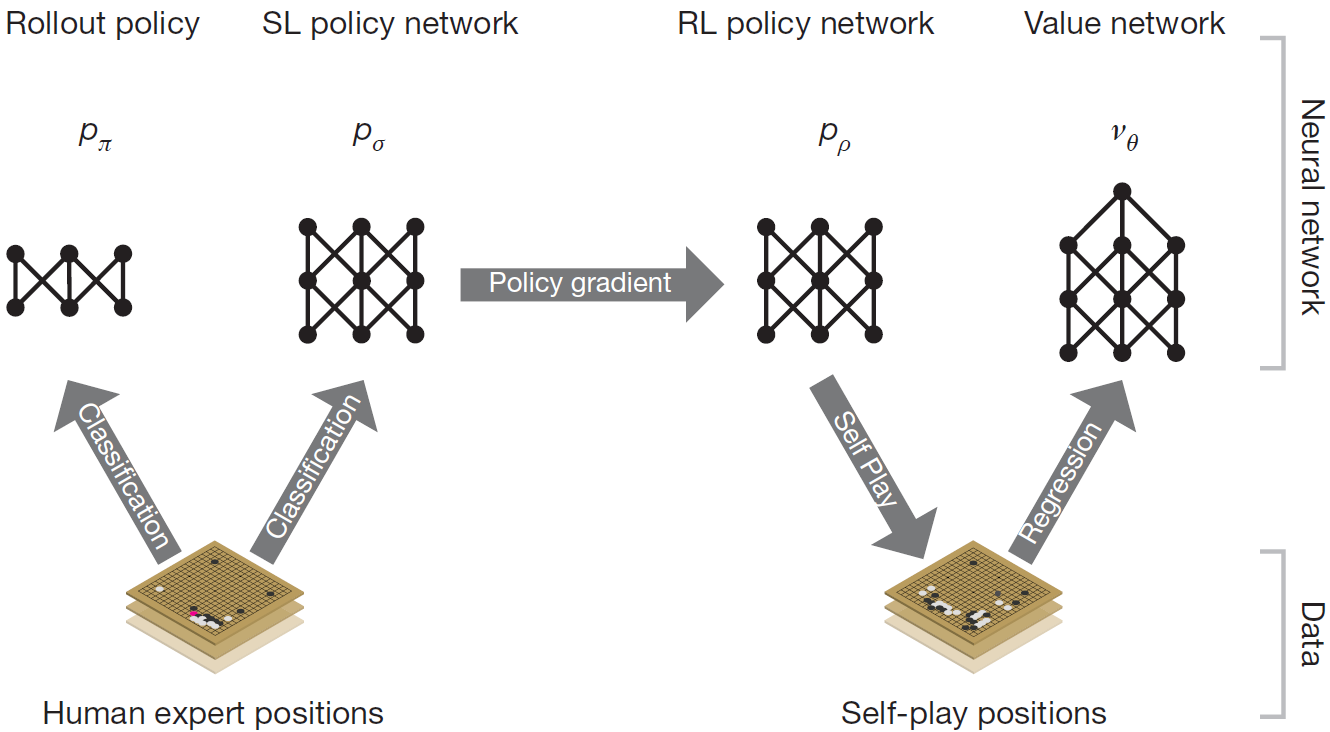
\includegraphics[width=\textwidth]{../img/neural_nets_pipeline.png}
      \end{center}
    \end{frame}

    \begin{frame}{ELO Ratings for~Various Combinations of~Networks}
      \begin{center}
        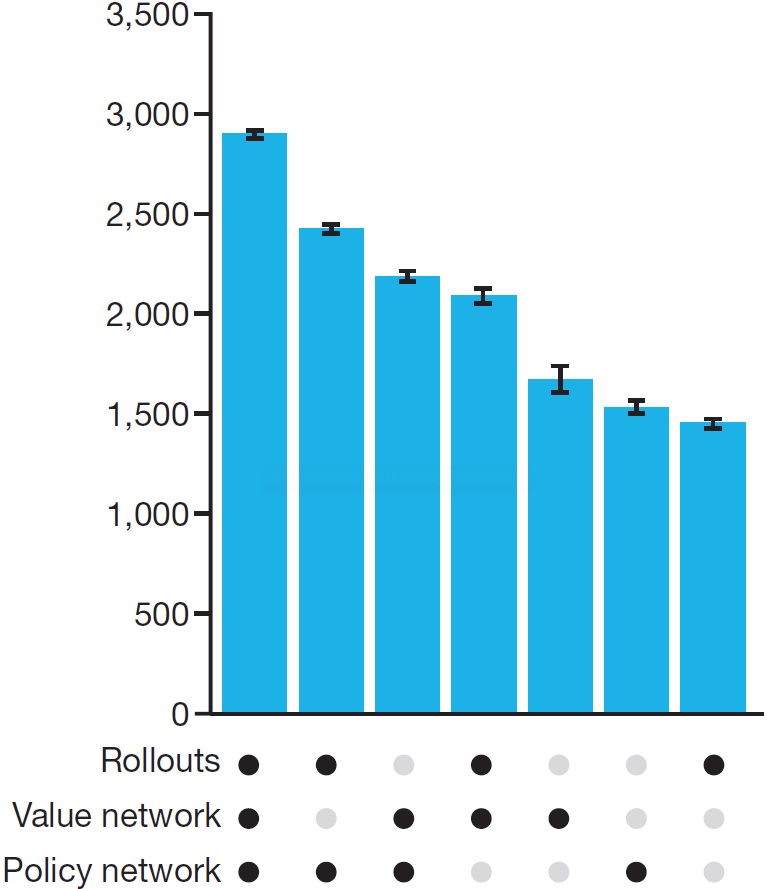
\includegraphics[height=.85\textheight]{../img/ELO_ratings_various_combinations_of_ANNs.png}
      \end{center}
    \end{frame}

    \begin{frame}{MCTS with Neural Networks (1/4)}
      \begin{center}
        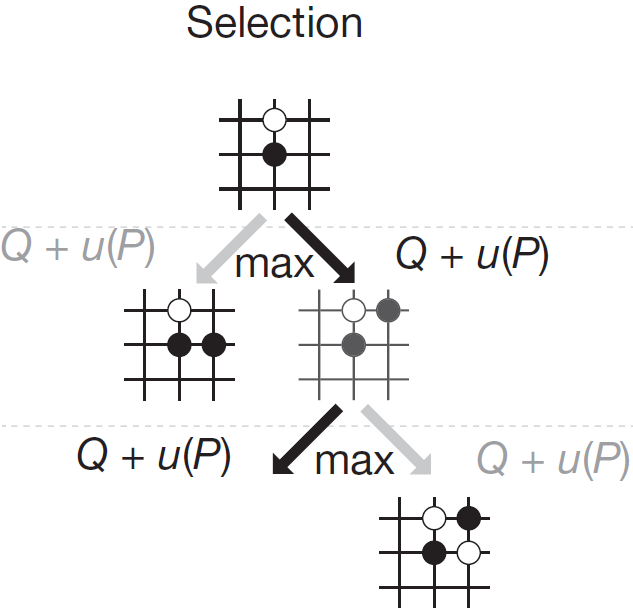
\includegraphics[height=.85\textheight]{../img/MCTS_selection.png}
      \end{center}
    \end{frame}

    \begin{frame}{MCTS with Neural Networks (2/4)}
      \begin{center}
        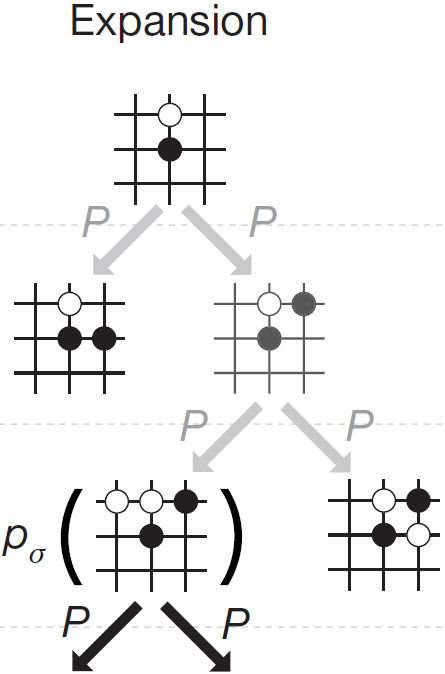
\includegraphics[height=.85\textheight]{../img/MCTS_expansion.png}
      \end{center}
    \end{frame}

    \begin{frame}{MCTS with Neural Networks (3/4)}
      \begin{center}
        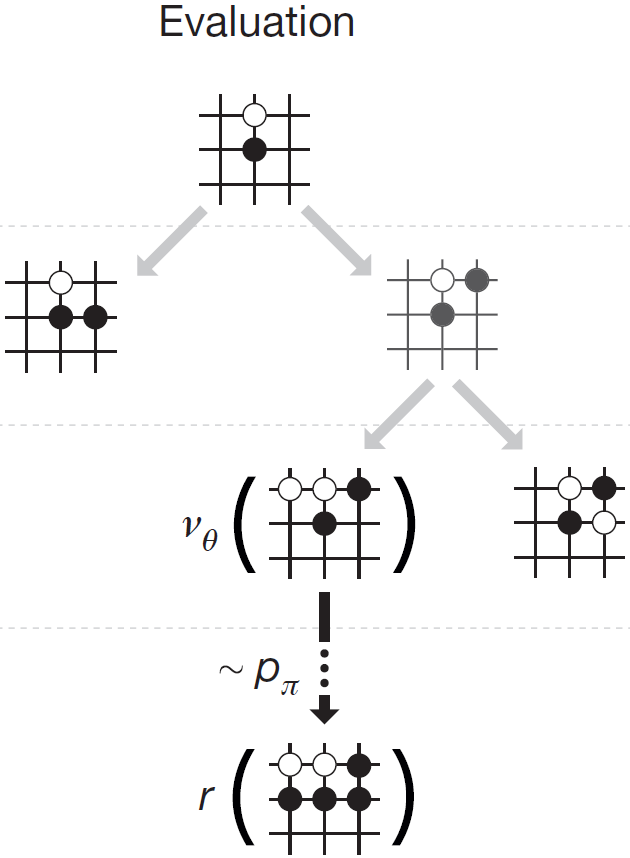
\includegraphics[height=.85\textheight]{../img/MCTS_evaluation.png}
      \end{center}
    \end{frame}

    \begin{frame}{MCTS with Neural Networks (4/4)}
      \begin{center}
        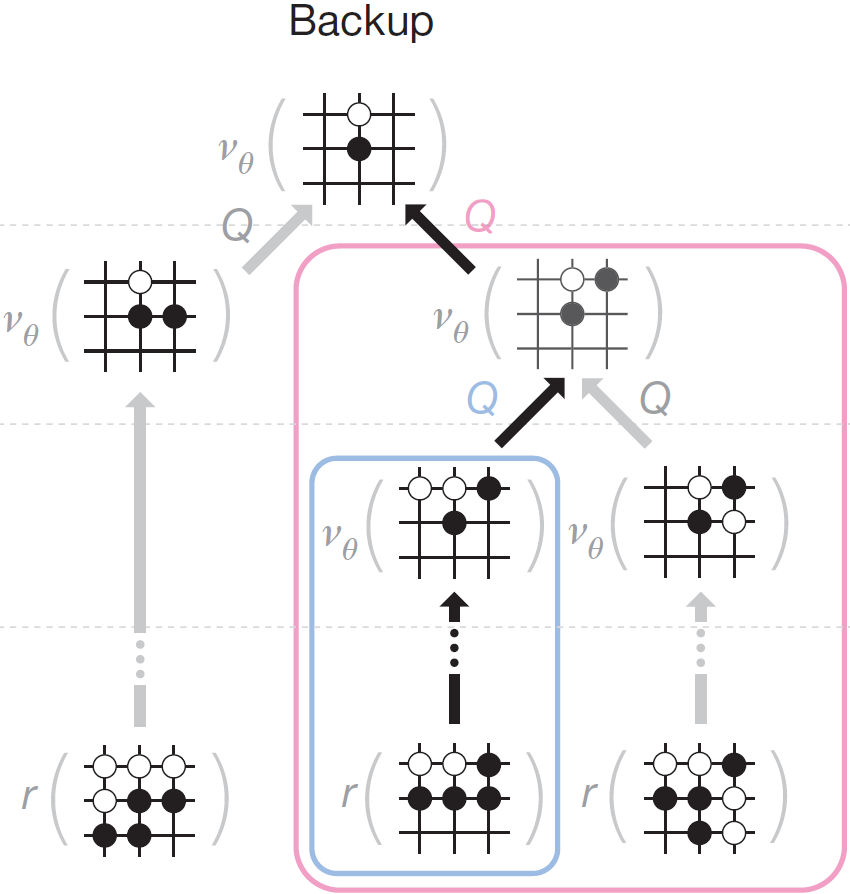
\includegraphics[height=.85\textheight]{../img/MCTS_backup.png}
      \end{center}
    \end{frame}

    \begin{frame}{Tree Evaluation from Value Network}
      \begin{center}
        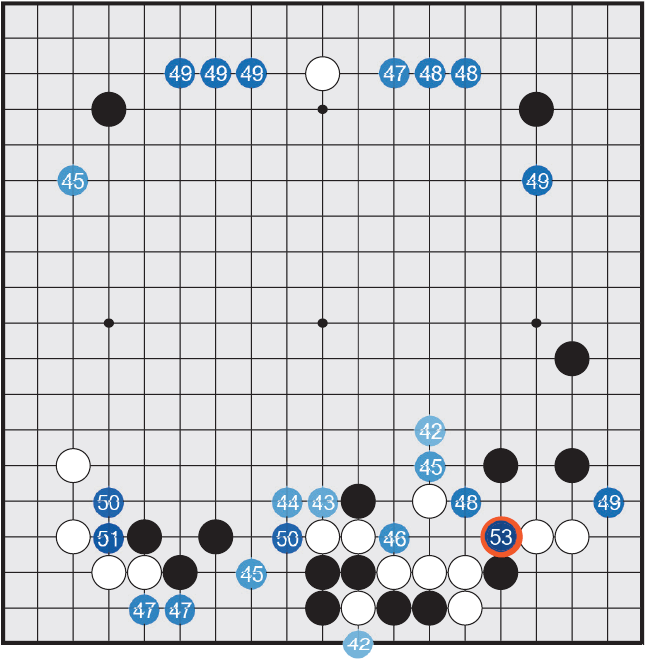
\includegraphics[height=.82\textheight]{../img/tree_eval_from_value_network.png}

        \tiny
        action values~$Q(s, a)$ for~each tree-edge~$(s, a)$ from root position~$s$ (averaged over value network evaluations only)
      \end{center}
    \end{frame}

    \begin{frame}{Tree Evaluation from Rollouts}
      \begin{center}
        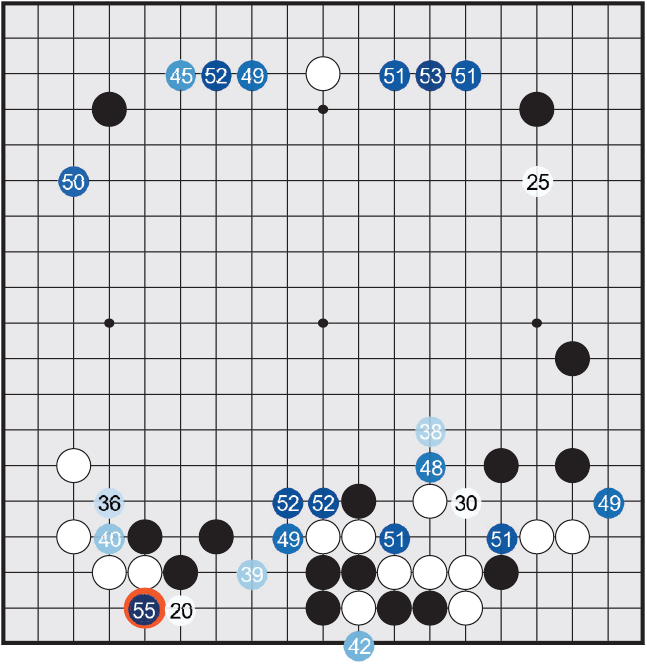
\includegraphics[height=.82\textheight]{../img/tree_eval_from_rollouts.png}

        \tiny
        action values $Q(s, a)$, averaged over rollout evaluations only
      \end{center}
    \end{frame}

    \begin{frame}{Percentage of~Simulations}
      \begin{center}
        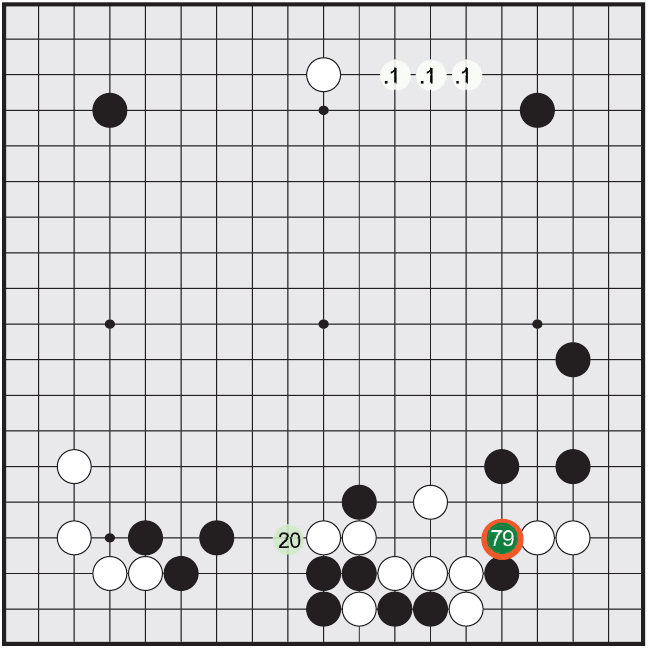
\includegraphics[height=.8\textheight]{../img/percentage_of_simulations.png}

        \tiny
        percentage frequency with which actions were selected from the root during simulations
      \end{center}
    \end{frame}

    \begin{frame}{Principal Variation (Path with Maximum Visit Count)}
      \begin{center}
        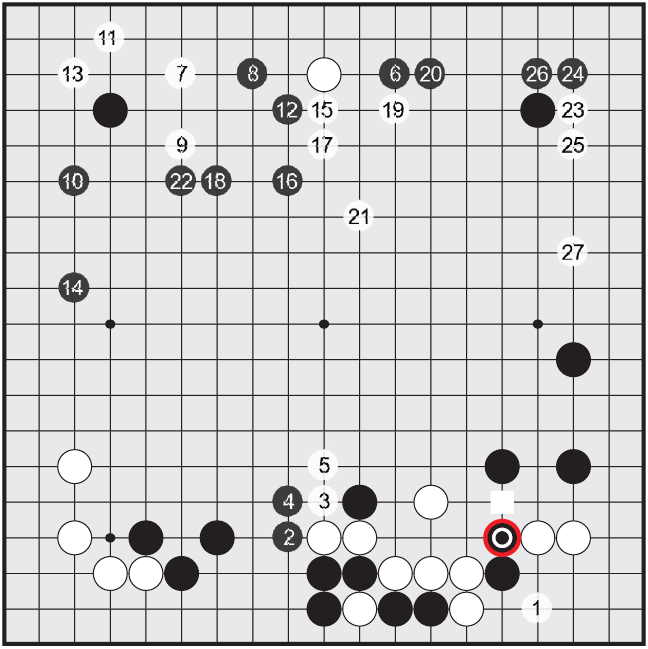
\includegraphics[height=.65\textheight]{../img/principal_variation.png}

        \tiny
        The moves are presented in a numbered sequence.
      \end{center}
      \pause

      \vskip -1ex
      \begin{tiny}
        \begin{itemize}[<+- | alert@+>]
          \item AlphaGo selected the move indicated by the red circle;
          \item Fan Hui responded with the move indicated by the white square;
          \item in his post-game commentary, he preferred the move (labelled 1) predicted by AlphaGo.
        \end{itemize}
      \end{tiny}
      \vskip 1.45em
    \end{frame}

    \begin{frame}{Scalability}
      \begin{itemize}[<+- | alert@+>]
        \item asynchronous multi-threaded search
        \item simulations on~CPUs
        \item computation of~neural networks on GPUs
      \end{itemize}
      \pause

      AlphaGo:
      \begin{itemize}[<+- | alert@+>]
        \item 40 search threads
        \item 40 CPUs
        \item 8 GPUs
      \end{itemize}
      \pause

      Distributed version of AlphaGo (on~multiple machines):
      \begin{itemize}[<+- | alert@+>]
        \item 40 search threads
        \item 1202 CPUs
        \item 176 GPUs
      \end{itemize}
    \end{frame}

    \begin{frame}{ELO Ratings for~Various Combinations of~Threads}
      \begin{center}
        \vskip -1ex
        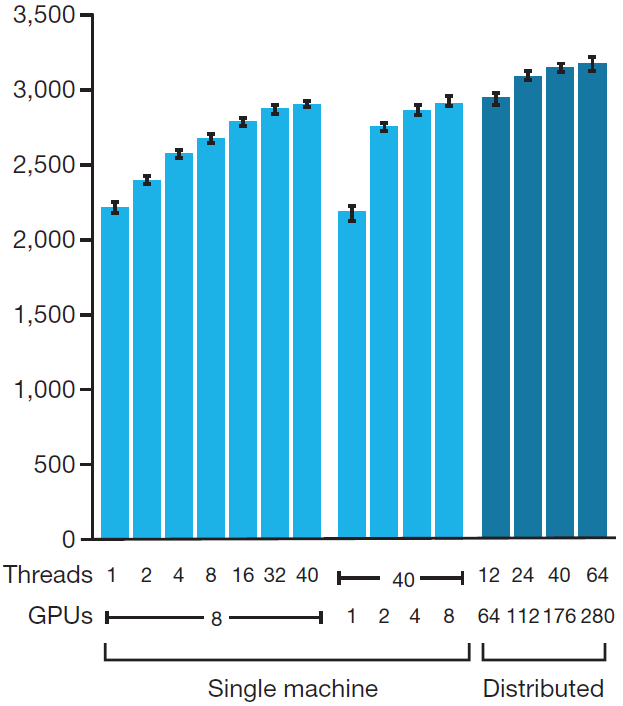
\includegraphics[height=.9\textheight]{../img/ELO_ratings_various_combinations_of_threads.png}
      \end{center}
    \end{frame}
  }

%%%%%%%%%%%%%%%%%%%%%%%%%%%%%%%%%%%%%%%%%%%%%%%%%%%%%%%%%%%%%%%%%%%%%%%%%%%%%%%%

  \section{Results: the strength of AlphaGo}

  {
    \setbeamertemplate{frame footer}{\cite{Silver2016mastering}}
    \begin{frame}{Tournament with Other Go Programs}
      \begin{center}
        \vskip -1ex
        \includegraphics[height=.95\textheight]{../img/results_of_tournament.png}
      \end{center}
    \end{frame}
  }

  {
    \setbeamertemplate{frame footer}{\url{https://en.wikipedia.org/wiki/Fan_Hui}}
    \begin{frame}{Fan Hui}
      \begin{center}
        \includegraphics[width=.55\textwidth]{../img/Fan_Hui_profile.jpg}
      \end{center}
      \pause
      \vskip -1.6em
      \begin{itemize}[<+- | alert@+>]
        \item professional 2 dan
        \item European Go Champion in 2013, 2014 and 2015
        \item European Professional Go Champion in 2016 
        \item biological neural network:
          \begin{itemize}[<+- | alert@+>]
            \item 100 billion neurons
            \item 100 up to 1,000 trillion neuronal connections
          \end{itemize}
      \end{itemize}
    \end{frame}
  }

  \begin{frame}{AlphaGo versus Fan Hui}
    \pause
    \begin{center}
      \includegraphics[width=.55\textwidth]{../img/Fan_Hui_loses.jpg}
    \end{center}
    \textbf{AlphaGo won 5 - 0} in a~formal match on~October 2015.
    \pause

    \vskip -1em
    \epigraph{
      \tiny
      [AlphaGo] is very strong and stable, it seems like a~wall.
      ...
      I know AlphaGo is a~computer, but if no one told me, maybe I would think the player was a~little strange, but a~very strong player, a~real person.
    }{Fan Hui}
  \end{frame}

  {
    \setbeamertemplate{frame footer}{\url{https://en.wikipedia.org/wiki/Lee_Sedol}}
    \begin{frame}{Lee Sedol ``The Strong Stone''}
      \begin{center}
        \includegraphics[width=.55\textwidth]{../img/Lee_Sedol_profile.jpg}
      \end{center}
      \pause
      \vskip -1.6em
      \begin{itemize}[<+- | alert@+>]
        \item professional 9 dan 
        \item the $2^{nd}$ in international titles
        \item the $5^{th}$ youngest (12 years 4 months) to become a~professional Go player in~South Korean history
        \item Lee Sedol would win 97 out of~100 games against Fan Hui.
        \item biological neural network, comparable to Fan Hui's (in~number of~neurons and connections)
      \end{itemize}
    \end{frame}
  }

  {
    \usebackgroundtemplate{
      \includegraphics[height=\paperheight]{../img/Lee_Sedol_quotes.jpg}
    }
    \begin{frame}[standout]
      \epigraph{
        \tiny
        I heard Google DeepMind's AI is surprisingly strong and getting stronger, but I am confident that I can win, at least this time.
      }{Lee Sedol}
      \pause

      \epigraph{
        \tiny
        ...even beating AlphaGo by 4-1 may allow the Google DeepMind team to claim its de facto victory and the defeat of him [Lee~Sedol], or even humankind.
      }{interview in JTBC Newsroom}
      \pause
    \end{frame}
  }

  {
    \usebackgroundtemplate{
      \includegraphics[height=\paperheight]{../img/Lee_Sedol_after_match.jpg}
    }
    \setbeamertemplate{frame footer}{\color{white}\url{https://en.wikipedia.org/wiki/AlphaGo_versus_Lee_Sedol}}
    \begin{frame}{AlphaGo versus Lee Sedol}
      \pause

      \vskip 1em
      \color{white}
      In March 2016 \textbf{AlphaGo won 4-1} against the legendary Lee Sedol.
      \pause

      AlphaGo won all but the $4^{th}$ game; all games were won by~resignation.
      \pause

      The winner of~the match was slated to win \$1 million.
      \pause

      Since AlphaGo won, Google DeepMind stated that the prize will be donated to~charities, including~UNICEF, and Go organisations.
      \pause

      Lee received \$170,000 (\$150,000 for participating in all the five games, and an additional \$20,000 for each game won).
    \end{frame}
  }

%%%%%%%%%%%%%%%%%%%%%%%%%%%%%%%%%%%%%%%%%%%%%%%%%%%%%%%%%%%%%%%%%%%%%%%%%%%%%%%%

  \section{Conclusion}

  \begin{frame}{Difficulties of~Go}
    \begin{itemize}[<+- | alert@+>]
      \item challenging decision-making
      \item intractable search space
      \item complex optimal solution
      
        {\tiny It appears infeasible to directly approximate using a~policy or value function!}
    \end{itemize}
  \end{frame}

  \begin{frame}{AlphaGo: summary}
    \begin{itemize}[<+- | alert@+>]
      \item Monte Carlo tree search
      \item effective move selection and position evaluation 
        \begin{itemize}[<+- | alert@+>]
          \item through deep convolutional neural networks
          \item trained by novel combination of~supervised and reinforcement learning
        \end{itemize}
      \item new search algorithm combining
        \begin{itemize}[<+- | alert@+>]
          \item neural network evaluation
          \item Monte Carlo rollouts
        \end{itemize}
      \item scalable implementation
        \begin{itemize}[<+- | alert@+>]
          \item multi-threaded simulations on CPUs
          \item parallel GPU computations
          \item distributed version over multiple machines
        \end{itemize}
    \end{itemize}
  \end{frame}
 
  \begin{frame}{Novel approach}
    \pause
    During the match against Fan Hui, AlphaGo evaluated \textbf{thousands of~times} fewer positions than DeepBlue against Kasparov.
    \pause

    It compensated this by:
    \begin{itemize}[<+- | alert@+>]
      \item selecting those positions \textbf{more intelligently} (policy network)
      \item evaluating them \textbf{more precisely} (value network)
    \end{itemize}
    \pause

    Deep Blue relied on a~handcrafted evaluation function.
    \pause

    AlphaGo was trained \textbf{directly and automatically} from gameplay.
    It used \textbf{general-purpose} learning.
    \pause

    This approach is not specific to the game of Go.
    The algorithm can be used \textbf{for much wider class} of~(so far seemingly) intractable problems in~AI!
  \end{frame}
  
  \begin{frame}[standout]
    \begin{center}
      Thank you!

      Questions?
    \end{center}
  \end{frame}

%%%%%%%%%%%%%%%%%%%%%%%%%%%%%%%%%%%%%%%%%%%%%%%%%%%%%%%%%%%%%%%%%%%%%%%%%%%%%%%%

  \appendix

  \begin{frame}[standout]
    Backup slides
  \end{frame}

  \begin{frame}{Further Reading}
    AI:
    \begin{itemize}
      \item \textbf{Singularity} \url{http://waitbutwhy.com/2015/01/artificial-intelligence-revolution-1.html} + Part 2
    \end{itemize}

    \todo
  \end{frame}

  \begin{frame}[allowframebreaks]{References}
    \tiny
    \printbibliography[heading=none]
  \end{frame}

\end{document}
